% New research manuscript. Earlier manuscripts and experimental outputs are unchanged.
% Compile main.tex with pdfLaTeX using the supplied Definitions/ directory.
\documentclass[jimaging,article,submit,pdftex,moreauthors]{Definitions/mdpi}
\usepackage{placeins}
\usepackage{longtable}
% Declare the same regular symbol fallback used by the template font stack.
\makeatletter\input{uwasy.fd}\makeatother
\DeclareFontShape{U}{wasy}{b}{n}{<->ssub * wasy/m/n}{}
\AtBeginDocument{\setlength{\headheight}{20pt}}
\usetikzlibrary{arrows.meta,positioning,fit,calc}
\firstpage{1}
\pubvolume{1}
\issuenum{1}
\articlenumber{0}
\pubyear{2026}
\copyrightyear{2026}
\externaleditor{}
\datereceived{}
\daterevised{}
\dateaccepted{}
\datepublished{}
\doinum{}
\Title{A Three-Dataset Evaluation of Flow Matching for Retinal Vessel Refinement with Native Patches and Nested Out-of-Fold Inputs}
\Author{Babak Bayanian $^{1}$, Hanieh Naderi $^{1,}$* and Chinthaka Dinesh $^{2,3,}$*}
\AuthorNames{Babak Bayanian, Hanieh Naderi and Chinthaka Dinesh}
\address{%
$^{1}$ \quad College of Interdisciplinary Science and Technologies, University of Tehran, Tehran 1439957131, Iran; babak.bayanian@ut.ac.ir\\
$^{2}$ \quad Department of Mechanical and Industrial Engineering, College of Engineering, Northeastern University, Vancouver, BC, Canada\\
$^{3}$ \quad School of Engineering Science, Simon Fraser University, Burnaby, BC, Canada}
\corres{Correspondence: hanieh.naderi@ut.ac.ir (H.N.); c.herathgedara@northeastern.edu (C.D.)}
\abstract{Flow Matching offers an iterative formulation for retinal vessel refinement, but its benefit must be separated from native image information and output selection. We report a three-dataset extension covering native-patch correction, nested out-of-fold (OOF) source maps, structural and preservation objectives, local acceptance and frozen whole-image context. Final comparisons use five matched correction-training seeds; shared upstream fits and single-fit pilots retain separate uncertainty units. Fresh three-fold evaluations cover 28 subject-grouped CHASE-DB1 images, 40 DRIVE images and 45 pathology-stratified HRF images. At the fixed 0.5 threshold, validation-selected Flow and capacity-matched direct controls preserve the native-patch direct refiner (O3) probabilities within the valid field of view, with mean Dice 0.815807, 0.800042, 0.759100, respectively. A validation-only calibration extension passes its prespecified gate on DRIVE and HRF. Relative to separately calibrated O3, Flow changes mean Dice by 0.000284 and 0.004872, clDice by 0.000282 and 0.006520, and thin-skeleton recall by 0.013709 and 0.033165, respectively. Flow-minus-Direct mean Dice is -0.000118 and -0.000435. Saved FP32 arrays support paired seed tests, Holm correction and exploratory cohort/seed intervals. Calibration exposes useful corrections, especially on HRF, while matched direct controls attain slightly higher mean Dice. Repeated validation use, shared upstream estimators and annotation-provenance limits keep these findings conditional; a Flow-specific or prospective clinical advantage is not established.}
\keyword{retinal vessel segmentation; probability-map refinement; flow matching; out-of-fold training; native-resolution patches; thin-vessel recall; clDice; paired evaluation}

\usepackage{needspace}

% Freeze the local draft date so the extracted Overleaf ZIP reproduces the PDF.
\renewcommand{\today}{November 19, 2026}
\begin{document}
\section{Introduction}\label{sec:introduction}
Retinal vessel segmentation is often summarized by an overlap score, although errors on small branches and errors on wider vessels have different spatial consequences. The public DRIVE, CHASE-DB1 and high-resolution fundus (HRF) datasets provide established settings for studying these problems, with differences in image resolution, population and annotation protocol~\cite{Staal2004,Fraz2012,Odstrcilik2013}. A model can recover additional vessel centreline pixels while adding false positives or altering vessel width. Conversely, a conservative prediction can obtain favorable precision while missing low-contrast branches. These competing outcomes make refinement of an existing probability map a useful setting for examining what a segmentation objective actually improves.

Encoder--decoder networks provide a standard foundation for biomedical segmentation~\cite{Ronneberger2015}. Retinal methods have further explored repeated refinement and explicit multiscale context~\cite{Li2020IterNet,Wu2021SCSNet}. A post-processing network conditioned on a coarse prediction and its red, green and blue (RGB) source image offers another route: the coarse model supplies a strong spatial prior, and the refiner can concentrate capacity on residual errors. This formulation also creates a preservation problem. A refiner can modify pixels that the coarse model already classified correctly, so the number of recovered vessels alone does not establish a beneficial overall change.

Flow matching learns a conditional vector field through a regression objective along prescribed paths~\cite{Lipman2023}; rectified flow studies a related transport formulation~\cite{Liu2023RectifiedFlow}. These frameworks motivate iterative segmentation refiners, but their generative interpretation does not by itself guarantee an improvement over a deterministic residual network. Recent flow-based work already addresses thin or curvilinear structures~\cite{Asadi2026FMS2,SidElMoctar2026CurvSegFlow}. The relevant question here is therefore empirical and narrower than proposing flow matching for vessels for the first time: under retained coarse inputs and fixed evaluation fields, which changes improve overlap, thin-vessel recovery, or both?

Our earlier study evaluated conditional diffusion refinement of lightweight U-Net with reverse attention (LU-Net+RA) probability maps~\cite{Bayanian2026}. The present work is a separate follow-up using a probability-grid reference-model family. Its initial phase compares three independently specified refinement recipes; subsequent phases test Flow corrections, stricter source construction, matched controls and validation-only connection screens, now extended to all three datasets. The first recipe adds missed-thin-vessel recovery and preservation losses to a deterministic Direct refiner. The second retains error-selective flow matching but supervises its full local endpoint and adds a preservation loss. The third retains the original Direct objective and trains on patches of native-resolution RGB images and annotations. The initial three recipes are evaluated separately; they are neither successive stages of one network nor an additive three-component architecture. The later development phases are identified separately rather than treated as additive contributions to one final model.

Training coarse maps are out of fold (OOF), whereas validation and test maps come from a fixed full-training baseline. Five refiner-training seeds are used per recipe and dataset. This arrangement isolates refiner variation conditional on the retained inputs; it does not constitute five independent repetitions of the entire segmentation pipeline. The experiments also have a sequential history: the objective study preceded the native-patch study, and the evaluation cohorts had already been examined. We preserve phase-specific validation locks and report the resulting comparisons as exploratory.

The contributions are as follows:
\begin{enumerate}[itemsep=0pt,parsep=0pt,topsep=3pt]
\item A three-dataset comparison of Direct objectives, endpoint-supervised Flow and native patches with matched coarse maps, ground truth (GT) and field of view (FOV).
\item Joint Dice, centreline Dice (clDice), thin-skeleton recall and precision reporting to measure both correction and damage.
\item A reproducible native-patch protocol with windowed residual fusion and projection to the unchanged comparison grid.
\item Source-bound five-seed summaries and paired uncertainty, with sequential selection and dependence made explicit.
\item Matched Flow/direct controls, nested OOF construction, dataset-appropriate fresh CV and three-dataset connection diagnostics, including negative results.
\end{enumerate}

In the initial nine-method phase, the native-patch recipe has the highest raw mean Dice on all three examined cohorts. The additional controls and sequential Flow follow-ups below test how that ranking changes under explicit preservation criteria and matched controls. This result has a clear qualification: the thin-recovery objective has higher thin-skeleton recall, and the original Direct control has higher precision. These outcomes motivate selecting a refinement objective and input recipe according to an explicit evaluation target rather than assuming that a more elaborate dynamical formulation or a structural loss will improve every measure.

% Expanded sections/related_work_2026-11-16_17-32-52.tex
\section{Related Work}
\label{sec:related_work}

\Needspace{8\baselineskip}
\subsection{Retinal Vessel Context and Structural Supervision}
Retinal vessel segmentation combines local appearance recognition with the recovery
of a spatially organized network. U-Net couples a contracting path with an expanding
path and skip connections to combine context and localization
\cite{Ronneberger2015}. Retinal applications have also used patch-based supervised
learning, including the deep networks of Liskowski and Krawiec
\cite{Liskowski2016}. These precedents mean that neither convolutional vessel
prediction nor patch-based processing is itself a new contribution. More recent
designs address the variation in vessel scale and surrounding anatomy explicitly.
For example, SCS-Net combines scale-aware aggregation, adaptive feature fusion and
multi-level supervision to model local detail and broader context
\cite{Wu2021SCSNet}.

Refinement can exploit relationships among vessel segments rather than treat every
pixel independently. IterNet uses repeated mini-U-Net processing, shared weights
and skip connections to infer obscured vessel details from intermediate
segmentations \cite{Li2020IterNet}. Structural supervision is another established
approach. The clDice measure compares segmentation masks with their centerlines,
and soft-clDice supplies a differentiable training surrogate
\cite{Shit2021}. These ideas motivate measuring more than overlap, but they do not
make the objectives interchangeable: centerline recovery, foreground precision and
whole-mask Dice can favor different predictions. Using a structural loss therefore
requires examining the resulting correction and damage, rather than assuming that
every vessel-related metric must improve.

\Needspace{8\baselineskip}
\subsection{Flow-Based Segmentation and Conditional Refinement}
Flow Matching trains a time-dependent vector field against prescribed conditional
paths, allowing transport to be learned without simulating the model trajectory
during training \cite{Lipman2023}. Rectified flow similarly learns transport along
straight interpolating paths and studies how rectification can simplify the
resulting trajectories \cite{Liu2023RectifiedFlow}. These formulations provide a
principled alternative to a single endpoint prediction. Their generative-modeling
results, however, do not establish an accuracy advantage for a particular retinal
refinement source, target or numerical solver.

Flow Matching has already been investigated for thin-structure segmentation. The
2026 FMS$^2$ preprint describes SegFlow, an image-to-mask transport model, alongside
a separate synthesis module \cite{Asadi2026FMS2}. The 2026 CurvSegFlow preprint
studies time-conditioned refinement for curvilinear structures and includes
retinal-vessel benchmarks among its evaluations \cite{SidElMoctar2026CurvSegFlow}.
Consequently, applying Flow Matching to thin structures or retinal vessels is not
the novelty claimed here. These methods also differ from the present fixed-coarse
refinement setup; their reported results are background evidence, not numerical
comparators under our retained splits and annotations.

Our earlier conditional-diffusion study evaluated refinement of LU-Net+RA
probability maps through a frozen encoded representation and found no mean-Dice
improvement under its documented protocol \cite{Bayanian2026}. That finding
motivates examining other refinement choices, but cannot establish a general
limitation of diffusion or Flow Matching. The present study instead compares
specific executable recipes: changing an objective at a common comparison
resolution, modifying endpoint supervision, and accessing native image detail
through a separate direct-refinement pipeline.

\Needspace{8\baselineskip}
\subsection{Native Patches, Fusion and the Scope of Comparison}
The benchmark sources provide complementary settings for this question. DRIVE
introduced a manually labeled retinal-image benchmark \cite{Staal2004}; CHASE-DB1
was introduced with an ensemble-based vessel segmentation study
\cite{Fraz2012}; and the HRF study provided high-resolution healthy and pathological
fundus images \cite{Odstrcilik2013}. Their original descriptions establish dataset
context, while the present source audit separately identifies the exact retained
annotations and conversions used in our experiments.

Patch processing offers access to image detail within a bounded memory footprint,
but introduces a reconstruction problem at patch boundaries. Pielawski and
W\"ahlby demonstrated that overlapping, window-weighted patch predictions can
reduce edge effects and studied Hann windows for this purpose
\cite{Pielawski2020}. Our residual fusion follows that established motivation;
Hann weighting itself is not presented as novel. A second distinction concerns
normalization. Group Normalization estimates moments within channel groups
\cite{Wu2018GroupNorm}; in our implementation, those moments are computed on each
tile. Thus, tiled processing changes spatial context and normalization support,
in addition to the sampling distribution and available resolution. Although the
sampled-pixel and optimizer-update budgets are matched to the original direct
control, the native-patch comparison remains a comparison of complete pipelines.
It cannot isolate a causal effect of resolution, and its projected 512-grid
evaluation does not constitute a native-grid accuracy assessment.

% Expanded sections/methods_v2_2026-11-16_17-32-52.tex
\section{Materials and Methods}\label{sec:methods}

\Needspace{8\baselineskip}
\subsection{Study Design, Data and Retained Coarse Predictions}
We investigate three refinement recipes: targeted thin-vessel recovery with
anchoring (O1), full-support endpoint supervision for selective Flow Matching
(O2), and native-resolution patch refinement (O3). Figure~\ref{fig:workflow}
summarizes these three paths. The frozen coarse predictor
is the executable LU-Net+RA reference associated with our previous conditional
diffusion study~\cite{Bayanian2026}. The initial three-recipe experiments use one retained
seed-42 baseline checkpoint per dataset, with 1,946,961 parameters and a
single-channel preprocessed input. No baseline or fold producer was retrained
for that initial phase; later nested-source and fresh subject-CV fits are
reported separately in Section~\ref{sec:sequential-methods}. The five retained control recipes described below are
separate previously completed experiments; their saved predictions remain unchanged; the combined analysis below independently replays their FP32 arrays.

Table~\ref{tab:protocol} specifies the fixed partitions. CHASE-DB1 keeps the two
eyes of each subject together throughout the outer split and cross-fitting
\cite{Fraz2012}. DRIVE uses its training/test partition with four training
images assigned to validation~\cite{Staal2004}. HRF is stratified into healthy,
diabetic-retinopathy and glaucoma categories, with 9/2/4 images per category in
training/validation/test~\cite{Odstrcilik2013}. Independent patient identifiers
were not established for DRIVE or HRF; their image-level partitions should not
be described as verified patient-disjoint partitions.

\begin{table}[htbp]
\caption{Fixed data protocol. Native dimensions are height $\times$ width.
OOF denotes out-of-fold coarse-map production within the outer training set.
FOV denotes field of view.
All comparative metrics use the original $512\times512$ grid.}
\label{tab:protocol}
\begin{adjustwidth}{-\extralength}{0cm}
\centering\small
\begin{tabularx}{\linewidth}{@{}lccccX@{}}
\toprule
Dataset & Native grid & Train/val/test & OOF folds & Test unit & Valid scoring region\\
\midrule
CHASE-DB1 & $960\times999$ & $16/4/8$ & 4 & 4 subjects & Whole image; two eyes per subject\\
DRIVE & $584\times565$ & $16/4/20$ & 4 & 20 images & Retained field-of-view mask\\
HRF & $2336\times3504$ & $27/6/12$ & 3 & 12 images & Retained JSON field-of-view bitmap\\
\bottomrule
\end{tabularx}
\end{adjustwidth}
\end{table}

Training coarse maps are retained OOF predictions from four subject-grouped
CHASE folds, four DRIVE image folds and three pathology-stratified HRF image
folds. Thus, 11 seed-42 fold checkpoints are reused. Fold fitting excludes the
held-out training images; checkpoint selection uses the outer validation set.
CHASE/DRIVE folds contain 12 fitting and 4 held-out images; HRF folds contain
18 fitting and 9 held-out images. Validation/test coarse maps instead come
from the corresponding full-training baseline. Checkpoint metadata, fold
inventories and exact prediction replay were checked, but this is not a fully
nested validation design or evidence that input-distribution shift is absent.

Coarse-predictor preprocessing applies green-channel contrast-limited
adaptive histogram equalization (CLAHE; clip limit 5,
$32\times32$ tiles), inverse-gamma correction with exponent $1/1.2$, and
bilinear resizing to $512\times512$. Refiner RGB inputs are divided by 255.
CHASE uses first-observer masks; DRIVE uses training manual1 GIFs and retained
local manual1 PNGs for test images. These labels are converted to luminance,
thresholded above 127 and resized with Pillow nearest-neighbour interpolation.
HRF vessels and field of view are reconstructed from indexed Supervisely
bitmaps at their recorded origins on the full canvas, then resized with OpenCV
nearest-neighbour interpolation. Native RGB, ground truth (GT) and FOV
dimensions agree for every
image, and their reference-grid conversions reproduce the retained tensors
exactly. A subsequent source-pixel audit is reported in Appendix~\ref{app:source-audit}.
It reconstructs all HRF targets from the official archive with a stated
white-only foreground rule, but does not recover the historical converter.
DRIVE images and training annotations were obtained from the Kaggle
repository \url{https://www.kaggle.com/datasets/andrewmvd/drive-digital-retinal-images-for-vessel-extraction}.
Test evaluation uses the retained local manual-1 PNG annotations.

\Needspace{8\baselineskip}
\subsection{Shared Refiner and Conditional Transport Representation}
Let $\mathbf{x}$ be RGB, $\mathbf{y}$ the binary reference,
$\mathbf{p}_0$ the frozen coarse probability map, and $V$ the valid-region
indicator. The source logits and full target are
\begin{equation}
\mathbf{a}_0=\operatorname{logit}\!\left(\operatorname{clip}
 (\mathbf{p}_0,10^{-4},1-10^{-4})\right),\qquad
\mathbf{a}_1^{\mathrm{full}}=6(2\mathbf{y}-1).
\label{eq:source-target}
\end{equation}
The spatial U-Net concatenates the current one-channel state, coarse map and
$2\mathbf{x}-1$. Four encoder widths are 12, 24, 48 and 96, with average-pool
downsampling, bilinear skip-connected decoding, two $3\times3$ convolutions
per block, four-group normalization and SiLU activations. A time embedding
contains $t$ and sine/cosine pairs at frequencies 1, 2, 4 and 8, followed by a
$9\!\to\!64\!\to\!64$ multilayer perceptron (MLP) and per-block
feature-wise linear modulation (FiLM). The one-channel head is zero
initialized; its output is multiplied by 6.

An auxiliary classifier receives coarse probabilities and RGB. Its two
12-channel convolutional blocks and final $1\times1$ convolution predict error
logits $\mathbf{g}_{\phi}$. Ungated recipes use the scaled U-Net velocity
directly; gated recipes multiply it by
$0.05+0.95\sigma(\mathbf{g}_{\phi})$. Hereafter $\mathbf{v}_{\theta}$ denotes
the velocity actually used, including this factor when applicable. All
recipes train 315,974 parameters, including the auxiliary classifier. Direct
deployment uses 314,185 velocity-network parameters; gated ESFM deployment
also uses the 1,789 classifier parameters. Balanced error supervision does
not establish calibrated error probabilities.

Define the training error mask
$E(u)=\mathbb{1}[\mathbb{1}[p_0(u)\geq0.5]\ne y(u)]$ and the selective target
\begin{equation}
\mathbf{a}_1^{\mathrm{sel}}
=(1-\mathbf{E})\odot\mathbf{a}_0
 +\mathbf{E}\odot\mathbf{a}_1^{\mathrm{full}}.
\end{equation}
For either target, the conditional linear path and local endpoint estimate are
\begin{equation}
\mathbf{z}_t=(1-t)\mathbf{a}_0+t\mathbf{a}_1,\quad
\mathbf{r}=\mathbf{a}_1-\mathbf{a}_0,\quad
\widehat{\mathbf{a}}_1=\mathbf{z}_t+(1-t)
\mathbf{v}_{\theta}(\mathbf{z}_t,t,\mathbf{p}_0,\mathbf{x}).
\label{eq:linear-path}
\end{equation}
This uses conditional vector-field regression~\cite{Lipman2023}. Iterative
recipes sample $t$ from $0.25\delta_0+0.75\mathcal{U}(0,1)$ during training;
Direct recipes set $t=0$. Inference starts deterministically at
$\mathbf{z}_0=\mathbf{a}_0$. Iterative recipes take eight Euler updates at
$t=k/8$, $k=0,\ldots,7$; the coarse/RGB condition is fixed and the gate is
computed once. Direct recipes take one residual update. No Gaussian initial
noise, reference error mask or skeleton is supplied at inference.

\Needspace{8\baselineskip}
\subsection{Shared Losses and Retained Controls}
The shared segmentation/classifier objective is
\begin{equation}
\mathcal{L}_{\mathrm{seg}}
=0.5\mathcal{L}_{\mathrm{BCE}}+0.5\mathcal{L}_{\mathrm{Dice}}
 +0.1\mathcal{L}_{\mathrm{soft\mbox{-}clDice}}
 +0.1\mathcal{L}_{\mathrm{gate}}.
\label{eq:shared-loss}
\end{equation}
BCE averages valid pixels after probabilities are clipped to
$[10^{-6},1-10^{-6}]$. Dice loss is averaged over images, using valid-region
probabilities and smoothing $10^{-6}$ in numerator and denominator.
Soft-clDice~\cite{Shit2021} uses the differentiable pooling skeleton with
iteration parameter 10: cross-shaped three-pixel erosion, $3\times3$ dilation
for opening, and accumulated nonnegative skeleton residuals. Its topology
precision/sensitivity ratios each add smoothing 1 to numerator and
denominator; their harmonic mean defines the per-image loss. GT is detached.
Gate BCE averages error and non-error class means equally over nonempty
valid supports within the minibatch.

Flow Matching additionally uses
\begin{equation}
\mathcal{L}_{\mathrm{FM}}=
\frac{\sum_u V(u)[1+4T(u)]
 [v_{\theta}(u)-r(u)]^2}
 {36\sum_u V(u)[1+4T(u)]},
\label{eq:fm-loss}
\end{equation}
where $T$ is the fixed training thin-skeleton support defined below and
$r(u)$ denotes the reference velocity at pixel $u$. Pixel sums extend across
the minibatch; Dice and soft-clDice are imagewise means.
The five retained controls are: (i) ordinary Direct, with the full target,
$t=0$, full-support segmentation loss and no FM loss; (ii) endpoint-supervised
iterative refinement, with the full target and sampled bridge states but no
FM loss; (iii) full-target ungated FM; (iv) selective-target ungated FM; and
(v) gated error-selective FM (ESFM). The last two use the training-only
auxiliary probability
$(1-\mathbf{E})\odot\mathbf{p}_0+
\mathbf{E}\odot\sigma(\widehat{\mathbf{a}}_1)$.
This composite holds correct pixels fixed only inside the auxiliary loss;
it does not constrain their deployed predictions. All five fit the auxiliary
classifier, even when it is unused at inference. Endpoint supervision is local,
not backpropagation through an unrolled eight-step solver.

\Needspace{8\baselineskip}
\subsection{O1: Missed-Thin Recovery and Correct-Pixel Anchoring}
O1 retains ordinary Direct and adds
$0.5\mathcal{L}_{\mathrm{thin}}+
\lambda\mathcal{L}_{\mathrm{anchor}}$ to Equation~\eqref{eq:shared-loss}.
Let $M=\{u:V(u)=1,T(u)=1,y(u)=1,p_0(u)<0.5\}$. Then
\begin{equation}
\mathcal{L}_{\mathrm{thin}}=
 |M|^{-1}\sum_{u\in M}\operatorname{softplus}(-\widehat a_1(u)).
\end{equation}
It returns zero for empty support. Correct thin pixels, non-thin misses and
invalid pixels do not enter this additional term. For correct foreground and
background supports $C_c=\{u:V(u)=1,\mathbb{1}[p_0(u)\geq0.5]=y(u)=c\}$,
the anchor is
\begin{equation}
\mathcal{L}_{\mathrm{anchor}}=
\frac{1}{|\mathcal{C}|}\sum_{c\in\mathcal{C}}
\frac{\sum_{u\in C_c}[\widehat p_1(u)-\operatorname{stopgrad}(p_0(u))]^2}{|C_c|},
\quad \mathcal{C}=\{c\in\{0,1\}:|C_c|>0\}.
\label{eq:anchor}
\end{equation}
Here $\widehat{\mathbf{p}}_1=\sigma(\widehat{\mathbf{a}}_1)$; nonempty class
means are equally weighted across the batch. With no correct pixels the
anchor is zero. This is a soft preservation preference, not an equality
constraint or an inference oracle.

\Needspace{8\baselineskip}
\subsection{O2: Full-Support Local Endpoint Supervision}
O2 retains the selective target, thin-weighted FM loss and learned gate of
ESFM, but evaluates all segmentation terms on
$\sigma(\widehat{\mathbf{a}}_1)$ throughout the valid region instead of the
error-mask composite. Its total objective is
$\mathcal{L}_{\mathrm{FM}}+\mathcal{L}_{\mathrm{seg}}
+\lambda\mathcal{L}_{\mathrm{anchor}}$.
There is no extra O1 thin-recovery term. Auxiliary gradients can therefore
oppose changes on initially correct pixels, while competing with their zero
target velocity. The supervised endpoint in Equation~\eqref{eq:linear-path}
comes from a reference-conditioned bridge state; it can differ from the final
Euler endpoint. Neither this change nor the nonzero-floor gate guarantees
non-degradation or topological preservation.

\Needspace{8\baselineskip}
\subsection{O3: Native-Resolution Patch Direct Refinement}
O3 preserves the ordinary Direct architecture and objective without FM,
missed-thin or anchoring terms. Native coarse inputs are bilinear projections
of the retained $512\times512$ OOF/full-baseline maps, with
\texttt{align\_corners=False}; they are not native-resolution baseline
predictions. Training uses four $256\times256$ patches per image per epoch.
Each centre is drawn with probability 0.5 from GT vessel pixels inside FOV,
otherwise uniformly from FOV; empty vessel support falls back to FOV. Crop
origins are clamped to the image boundary. Coarse, RGB, GT and FOV receive
identical right-angle rotations and horizontal/vertical flips. Native GT is
used only for fitting patches, not for the reported comparative metrics.

Inference tiles native RGB/coarse inputs with size 256, stride 128 and a final
tile anchored to each image edge. A positive separable Hann window, whose
one-dimensional weights are floored at $10^{-3}$, averages overlapping logit
residuals~\cite{Pielawski2020}. There is no halo, and GroupNorm uses tile-local
statistics. The resulting native residual $\mathbf{d}$ is projected to the
comparison grid by the dataset's GT nearest-neighbour rule: Pillow float-image
nearest for CHASE/DRIVE, OpenCV nearest for HRF. The primary output is
\begin{equation}
\mathbf{p}_{\mathrm{raw}}=
\sigma\!\left(\mathbf{a}_0+R_{\mathrm{NN}}\mathbf{d}\right).
\label{eq:native-projection}
\end{equation}
Only the residual is projected; downsampling the native probability would
resample the frozen baseline. Exact zero residuals return the original coarse
probability to avoid a single-precision floating-point (FP32) logit/sigmoid
rounding change. This inference
branch is absent from the differentiable training loss.

\paragraph{Deployment procedure.}
\begin{enumerate}
\item Fix RGB and the coarse map. O1 applies one Direct update; O2 computes
its gate once and performs eight Euler updates, retaining the same condition.
\item For O3, evaluate overlapping native tiles, fuse logit residuals and
apply Equation~\eqref{eq:native-projection} on the original comparison grid.
\item Apply the locked secondary blend if required. Prediction uses no GT,
reference skeleton or error mask; evaluation subsequently applies threshold
0.5 and the fixed valid-region convention.
\end{enumerate}

\Needspace{8\baselineskip}
\subsection{Initial-Phase Fitting and Selection}
The initial O1/O2/O3 comparisons use five independent refiner training seeds:
42, 123, 2026, 3000 and 3001. Each fit uses 120 epochs, FP32, AdamW with initial
learning rate $3\times10^{-4}$ and weight decay $10^{-4}$, cosine annealing,
and separate velocity/classifier gradient-norm clipping at 1. No learning-rate
warm-up is used. O1/O2 and retained controls use batches of four full
$512\times512$ images. O3 uses 16 native patches per batch, matching sampled
pixels and optimizer updates: four updates per epoch for CHASE/DRIVE and
seven for HRF. This does not match sampling distributions, context,
normalization or inference cost.

O1/O2 first compare $\lambda\in\{0.1,1.0\}$ using pilot seed 91011, separately
for each recipe/dataset. The 12 pilot fits select the best learned validation
Dice checkpoint among epochs 10--120, evaluated every ten epochs. Improvements
must exceed $10^{-12}$; ties retain the smaller anchor and earlier epoch.
The resulting anchors are 1.0 for O1 and 0.1 for O2 on all datasets. All six
configurations were locked before 30 fresh final fits, and all 30 final
raw/blend choices were locked before V3 test scoring.

O3 is a later follow-up on already examined cohorts, with fixed patch settings
and no additional pilot search. Its 15 final choices were separately locked
before O3 test scoring. There was no single 45-model lock preceding all phases.
Thus, 57 completed new fits comprise 12 development pilots and 45 final fits;
75 retained control fits are additional reused evidence. An interrupted
28-epoch native attempt completed no fit or test evaluation and contributed
no weights or results to the restarted study.

For each final fit, raw validation mean image Dice selects a learned epoch;
identity is excluded. Secondary blending independently selects epoch and
$\alpha\in\{0,0.25,0.5,0.75,1\}$ for
$(1-\alpha)\mathbf{p}_0+\alpha\mathbf{p}_{\mathrm{raw}}$, including exact
baseline identity at epoch zero. These rules do not undo prior test exposure
or make O1/O2's additional pilot search equivalent to control development.
Reported training used PyTorch 2.11.0, CUDA 12.6 and an RTX 4070 Ti SUPER.


\Needspace{8\baselineskip}
\subsection{Completed Sequential Experiments}\label{sec:sequential-methods}
The initial controls and O1/O2/O3 recipes are separate from the subsequent
F1--F9 development sequence. Applying Flow Matching to retinal vessels is not
claimed as a first use. Each phase has its own input lineage and validation
history. The later missing-dataset extension uses new dataset-specific
validation records, not a retrospective global lock over previously seen tests.
Previously inspected cohorts and repeated validation use make these exploratory
comparisons. No earlier prediction, checkpoint or manuscript is replaced.
The earlier encoded-flow pilot and AE-free mask-grid prototype use in-sample
coarse maps; they precede the OOF recipe series and are labelled separately.
The encoded pilot is one trained model with five initial-noise realizations.
The mask-grid prototype instead has five independently initialized refiner fits.

F1 trains an AE-free native-patch Flow for 120 epochs with 8 Euler updates.
F2 retains a frozen full-training O3 anchor and learns a zero-initialized bounded
Flow field; four 40-epoch pilots compare caps 1/2 and FM coefficients 0.01/0.1,
followed by five 120-epoch fields. Validation selects checkpoint and strength
from 0,0.25,0.5,1; strength 0 is exactly the retained O3 prediction. Raw strength 1
is separate. Solver/path diagnostics use validation only. F3 instead obtains
every training O3 input from a whole-chain nested exclusion: an O3 model
excludes the input's group, and each of its fitting coarse producers excludes
both that held group and the fitting input's own group. The deployed O3 remains
the retained full-training model. Four groups are used for the new nested
HRF source chain, distinct from its original three-fold coarse-map recipe.

F4 adds native and exactly aligned 512-grid structural supervision. PIL nearest
indices are used for CHASE/DRIVE; HRF uses the original OpenCV nearest indices.
Four 40-epoch cap/structure pilots precede five 120-epoch fits. Its original
selection permits a Dice decrease of 0.0005 and a precision decrease of 0.002;
this rule is not renamed Dice preservation. F5 evaluates four signed-field
pilots and four warm-start retention pilots before five 120-epoch fits. Its
selection disallows Dice decrease, retains a 0.002 precision tolerance and ranks
retention of prior structural gain. Depending on the validation-selected family,
the final seeds are signed-field fits or warm fine-tunes of the five matched
F4 fields. A warm epoch-zero choice reuses the retained field rather than
establishing a new learning improvement. A 24-point validation-only strength/bias
probe is reported separately and is not a test-selected replacement.

F6 operates on the 512 grid with GT-free geometrical regions, matched Flow/direct
local proposers and a learned acceptance critic. Four auxiliary proposer fits
per arm use pair-excluded O3 inputs; their held-group proposals supply critic
targets. Pair-excluded O3 fitting inputs require triple-excluded baselines.
These baselines retain the 200 optimizer-update minimum and validation-softDice
tie break. Eight auxiliary 80-epoch proposers, ten final 120-epoch proposers and
ten 100-epoch critics are used per dataset. The shared auxiliary seed is 91011.
Validation calibrates strength and critic conservatism; identity remains
eligible. The critic predicts changes in Dice, clDice and thin recall. Its
three-metric acceptance rule does not guarantee precision or test improvement.

F7 uses native 256 patches, on-policy rollout supervision and matched direct
fields; two 80-epoch preservation pilots precede five 80-epoch pairs. F8 adds
frozen ImageNet ResNet18~\cite{He2016} whole-image features to both arms. Its encoder is not
fitted on retinal labels. Context is extracted from the full RGB field resized
to 224 square with ImageNet normalization, without a centre crop. Both arms use
the same initialized trainable capacity, crop/augmentation draws and image
budget. Flow uses more field evaluations; parameter matching is not compute
matching. F7/F8 search 2/4/8 Flow steps versus one direct call, so their candidate
counts are not generally matched. Their pilots use seed 42, which also appears
among the five final seeds; pilot fits are not additional independent repeats.
The F7 direct arm inherits the preservation
coefficient chosen by the Flow pilot. For F7--F9, the raw row is the
validation-ranked learned candidate across checkpoints, strengths and solver
settings without requiring the preservation gate; it need not use strength 1.
The selected row requires the phase-specific gate or returns identity.
F7/F8 retain their original three-metric validation eligibility
rule. The requested missing-dataset five-seed comparisons are completed even
when their pilot fails; unqualified deployed outputs remain exact identity.
Geometry-guided Flow retains the one 80-epoch seed 42 pilot scope used on CHASE;
it is not presented as a five-seed result. FR-UNet~\cite{Liu2022FRUNet} likewise retains three
validation-learning-rate pilots per dataset. Its official one-channel network
uses the retained 512 green fields, full-image BCE, Adam with weight decay
$10^{-5}$, a 120-epoch cosine schedule and learning-rate candidates
$10^{-5},10^{-4},3\times 10^{-4}$. The logical batch is 4 with microbatch 1;
BatchNorm statistics use microbatch 1. Dual-threshold iteration is not executed.
The official SegFlow adaptation uses its existing five EMA checkpoints,
RGB inputs resized to 256, zero initial self-conditioning and ten Euler updates
starting from the RGB state, followed by the fixed 512 probability projection.
Its missing HRF test outputs are generated without
retraining. These are local protocol adaptations, not reproductions of the
external papers' reported benchmark scores.

\Needspace{8\baselineskip}
\subsection{Nested Source Exclusion}
Let $\mathcal{T}$ be a fitting partition and $G_k$ one of its four inner
groups. The baseline operator $B$ includes the unchanged image preprocessing.
An O3 source model excluding $G_k$ is fitted using nested coarse inputs:
\begin{equation}
b_u^{-(k,j)}=B_{-(k,j)}(I_u),\quad u\in G_j,\ j\ne k,
\qquad
p_i^{\mathrm{OOF}}=\mathrm{O3}_{-k}\bigl(I_i,B_{-k}(I_i)\bigr),\quad i\in G_k.
\label{eq:nested-source}
\end{equation}
Subscripts list excluded groups, rather than random seeds. Thus the labels of
$i$ are absent from the O3 source fit, its checkpoint-selection inputs and
every coarse producer used to fit that O3 model. External validation images
remain outside $\mathcal{T}$. For F6's pair-excluded critic source
$\mathrm{O3}_{-(k,j)}$, a fitting image in $G_l$ instead receives a coarse map
from $B_{-(k,j,l)}$. The stored lineage records enumerate these actual sets;
merely using a final held-image prediction is insufficient to establish
indirect exclusion. Each source stores aligned native and comparison-grid
fields, with the residual projected onto the original coarse map. In fresh
outer CV, the outer-test images are additionally excluded from all the above
fits and validation decisions.

\Needspace{8\baselineskip}
\subsection{Executable Rollout and Context Correction}
For F7--F9, let $p^n$ denote a frozen native O3 field and $c$ the optional
same-image frozen RGB context. The correction state starts at zero, and its
implemented Euler updates are
\begin{equation}
r_0=0,\qquad
r_{j+1}=r_j+\frac{1}{S}v_\theta(r_j,j/S,p^n,I,c),\qquad
v_\theta=6\tanh\!\left(f_\theta/6\right).
\label{eq:correction-rollout}
\end{equation}
Training unrolls four steps. Validation searches $S\in\{2,4,8\}$ for Flow;
the matched direct control uses the same initialized field architecture in a
single call at state and time zero. These phases use deterministic inference
conditional on the fitted weights and locked choices, with no initial-noise
sampling. Positive-Hann fusion of native patch corrections is followed by the
dataset's recorded nearest projection $\mathcal{P}_{512}$. Writing the final
comparison-grid residual as $q=\beta\mathcal{P}_{512}(r)$, inference preserves
the original O3 probability exactly wherever the correction is zero:
\begin{equation}
p^*(x)=
\begin{cases}
p^{512}(x),&q(x)=0,\\
\sigma\!\left(\operatorname{logit}_{\epsilon}(p^{512}(x))+q(x)\right),&q(x)\ne 0,
\end{cases}
\qquad \epsilon=10^{-4}.
\label{eq:correction-output}
\end{equation}
Here $\operatorname{logit}_{\epsilon}$ clips its probability argument to
$[\epsilon,1-\epsilon]$. This zero-residual branch prevents an FP32
logit/sigmoid round trip from changing a threshold tie.

Each fitting image supplies four augmented native 256 patches per epoch.
Requested crop-centre strata are missed-thin 40\%, near-false-positive 25\%,
correct-thin 20\% and random-valid 15\%; an empty stratum falls back to valid
random pixels. Only training GT defines these sampling supports. Matched arms
share crop draws, rotations by multiples of $90^\circ$ and horizontal/vertical
flips. Optimization uses AdamW with
learning rate $3\times 10^{-4}$, weight decay $10^{-4}$, cosine decay without
warm-up, gradient clipping at 1 and effective batch 8 with microbatches 4.
Inference uses 256 tiles, stride 128 and batch 8, with strictly positive Hann
weights. The full-image context and every inference input remain GT-free.

For training only, the expert residual is the clipped correction toward
margin $1.5$, restricted to erroneous O3 pixels:
\begin{equation}
r^*=\mathbf{1}_{\{(p^n\geq 0.5)\ne g\}}
\operatorname{clip}\!\left(1.5(2 g-1)-\operatorname{logit}_{\epsilon}(p^n),-6,6\right).
\label{eq:rollout-expert}
\end{equation}
Conditional field regression samples the straight state $t r^*$ and target
$r^*$. The additional on-policy imitation term uses a detached model state
after two of four Euler updates and a clipped remaining-velocity target
$\operatorname{clip}((r^*-r_{1/2})/0.5,-6,6)$. This imitation term is
distinguished from conditional Flow Matching itself. Both controls share the
endpoint, preservation and structural terms; the two field-regression terms
apply only to Flow. With $n$ and $e$ denoting native and aligned evaluation
grids, respectively, the implemented objective is
\begin{equation}
\begin{aligned}
\mathcal{L}={}&0.05\mathcal{L}_{\mathrm{FM}}+0.05\mathcal{L}_{\mathrm{on}}
+0.125(B_n+B_e)+0.25(D_n+D_e)\\
&+0.5\mathcal{L}_{\mathrm{structure}}+\lambda_P\mathcal{L}_{\mathrm{preserve}}
+2(R_n+R_e),\\
\mathcal{L}_{\mathrm{structure}}={}&\tfrac 12\bigl[(C_n+0.5 T_n+0.25 K_n)
+(C_e+0.5 T_e+0.25 K_e)\bigr].
\end{aligned}
\label{eq:rollout-objective}
\end{equation}
$B$ is the class-balanced BCE term, $D$ soft-Dice loss, $C$ soft-clDice loss,
$T$ positive-skeleton softplus loss and $K$ skeleton/near-background BCE.
$R$ penalizes a soft-Dice loss exceeding the source's loss. Preservation
combines a sign-margin hinge with a $0.25$ probability-change penalty on
correctly classified source pixels, balanced between foreground and background
and averaged across the two grids. F7 tests $\lambda_P=1$ and $4$ using its
two validation pilots; F8/F9 use $1$. Native thin training support has EDT
radius at most two native pixels; aligned comparison-grid support uses the
fixed one-pixel cutoff. Structural training uses ten soft-skeleton iterations
and excludes a three-pixel crop boundary. These training surrogates differ
from the full-image hard evaluation skeletons. GT supplies training targets
and losses only; it is absent from correction inference.

\Needspace{8\baselineskip}
\subsection{Fresh Outer Cross-Validation and Precision Guard}
F9 uses three outer folds. CHASE retains subject grouping over 28 images;
DRIVE uses all 40 retained images with native-size annotations and image-level
folds; HRF uses 45 images stratified by pathology. DRIVE/HRF patient linkage is
unverified, so their folds are not called patient-disjoint. DRIVE reserves four
inner-validation images per fold; HRF reserves two per pathology. Each outer
training set has four inner OOF groups. Each outer fold fits one full,
four single-exclusion and six pair-exclusion baselines, then one full and
four excluded-group O3 models. Across three folds this gives 33 baseline and
15 O3 fits per dataset. Five correction seeds then share each fold's upstream
models: these are 30 correction fits, not five complete pipeline repetitions.
Outer-test images are excluded from every fitting and checkpoint-selection
dependency. No retinal checkpoint from the earlier fixed split initializes this
fresh chain; only the frozen ImageNet context is reused.

The F9 candidate must preserve validation Dice and precision (tolerance
$10^{-12}$) and strictly improve both clDice and thin recall. It maximizes mean
structural gain; otherwise the selected output is exactly O3. All 30 correction
choices are locked before fresh-pipeline outer-test inference. The fixed-cohort F8
checkpoints also receive a separate retrospective validation precision-guard
re-selection, without retraining. Threshold calibration mirrors the original
single-seed three-fold diagnostic: epochs 20/40/60/80, four strengths,81 thresholds
from 0.10 to 0.90, and matched Flow/direct evaluation. Average precision excludes
pixels outside FOV. AP-max configurations are optimistic validation diagnostics,
not evidence of test gain. The original aggregate four-metric pilot gate
determines whether the remaining four stored correction seeds are calibrated
and evaluated. All 30 choices are then locked before the new calibrated outer
evaluation; calibration-only O3 gains are never credited to Flow.
Connection-repair diagnostics compare GT-free
candidate tubes, an unfiltered union and an explicitly GT-filtered oracle;
oracle gains never count as a trained Flow result.

\Needspace{8\baselineskip}
\subsection{Outcomes, Statistical Units and Verification}
Fixed-threshold primary scores use the unchanged 512-grid GT and probability threshold
$p\geq 0.5$, with the original valid FOV. Thin support is the GT skeleton with
padded Euclidean distance-transform radius at most one evaluation-grid pixel.
It is an operational thin-vessel definition, not a calibrated anatomical width.
The separate calibration comparison uses its locked fold-specific thresholds.
Soft training skeletons and hard evaluation skeletons are different quantities.
IoU, recall, specificity, accuracy, skeleton precision/sensitivity, correction
and damage rates and component-count discrepancy are supplied as secondary
descriptive seed summaries; primary test families retain the four stated outcomes.
FP32 probabilities, GT and FOV are reopened before independent metric replay;
raw, selected and identity outputs are kept distinct. Initial-noise repetitions
of one encoded model are averaged as metrics and are not independent trainings.
Native-resolution validation probes do not replace primary 512-grid scores.
The word raw retains each phase's recorded rule: fixed-final encoded/mask
prototypes; validation-chosen unblended initial/F1 checkpoints; strength 1
F2--F5 fields; and the F6 strength 1 proposer before critic acceptance. Newly
exported F7--F9 raw rows are the validation-ranked diagnostic candidate,
including its recorded checkpoint, strength and solver. They are not assumed
to be fixed-final or strength 1 outputs. Their earlier CHASE raw counterparts
were not exported and are not invented.

Means and sample SDs describe the five matched training-seed means. Paired
two-sided t intervals use four degrees of freedom. Exact two-sided signed-rank
tests are separate; with five nonzero concordant pairs their minimum attainable
p value is 0.0625. An all-zero identity contrast has interval[0,0] and p=1;
it does not establish equivalence. Newly combined Holm families are declared by
cohort, phase, arm/output and contrast across the available dataset/metric cells;
the full-precision tables include family membership and size. Direct/Flow
comparisons use matched seeds, source images and exact input hashes.
Recipe-specific controls use their matched retained control, and factorial
interactions are kept separate. Exploratory adjacent-recipe contrasts compare
F2 with F1 raw, F3 with F2 selected, F4 with F3 selected, F5 with F4 selected,
and each F8 arm with its corresponding F7 arm. These are paired system
comparisons; changes in source, capacity, objective or selection prevent a
single-factor causal interpretation. Historical single-dataset p values are not
silently relabelled as corrected over newly added datasets.

Exploratory crossed bootstrap intervals use 50,000 seed/cohort resamples with
seed 20261118. CHASE resamples subjects with both eyes; DRIVE/HRF resample
images. Resampling preserves outer-fold strata and HRF pathology strata.
These intervals are conditional on the retained cohort, source fits and
selection history; they are not prospective clinical confidence bounds.
The exploratory inference is not rescued by treating dependent patches,
pixels, sampling seeds or critic offers as additional independent subjects.
All loss and checkpoint settings are fixed or validation-selected, never chosen
by test performance. Negative results and exact fallback remain in the tables.

\Needspace{8\baselineskip}
\subsection{Computational Provenance and AI Assistance}
The extension retains FP32 execution, disabled TF 32, deterministic cuDNN
settings and disabled cuDNN benchmarking. These recorded settings are not a
claim that every training operation is bitwise reproducible across software
versions or devices. Independent DRIVE work overlaps the primary HRF worker;
frozen-model validation diagnostics also overlap fitting when memory permits.
Each process has separate random generators, selection records and output
paths. No overlapping-job wall time is reported as an isolated latency
benchmark. Source versions, initialization and crop checks, checkpoint hashes
and saved predictions accompany the execution records. The large number of
source, pilot and final fitting calls is not an inferential sample size.
OpenAI Codex assisted implementation, workflow orchestration, verification and
drafting. Scientific plots use Matplotlib and real saved arrays; the schematic
uses TikZ. Exact AI-version and author-disclosure details remain subject to
the author confirmations stated in the acknowledgments.
\begin{figure}[H]
\begin{adjustwidth}{-\extralength}{0cm}
\centering
% Expanded figures/workflow_three_options_v2_2026-11-16_17-32-52.tex
% TikZ snippet; load arrows.meta,positioning,fit,calc. No outer float.
\begin{tikzpicture}[font=\small,>=Latex,
 box/.style={draw=black!60,rounded corners=2pt,align=center,text width=4.9cm,minimum height=1.15cm,inner sep=5pt},
 link/.style={->,line width=.65pt},
 note/.style={align=center,text width=16.8cm,font=\footnotesize}]
\node[box,text width=16.8cm,fill=gray!7] (input) {Fixed baseline seed 42 and retained out-of-fold training maps\\Frozen 512-grid coarse probabilities; aligned RGB, ground truth and FOV};
\node[box,below=8mm of input,xshift=-5.9cm,fill=blue!5] (o1) {\textbf{Option 1: Direct objective}\\512-grid refiner\\Missed-thin recovery + correct-pixel anchor};
\node[box,below=8mm of input,fill=green!5] (o2) {\textbf{Option 2: ESFM objective}\\512-grid refiner\\Full-support endpoint loss\\+ correct-pixel anchor};
\node[box,below=8mm of input,xshift=5.9cm,fill=orange!8] (o3) {\textbf{Option 3: Native patches}\\Native RGB/GT/FOV; $256\times256$ crops\\Unchanged Direct loss};
\draw[link] (input.south) -- ++(0,-3mm) -| (o1.north);
\draw[link] (input.south) -- (o2.north);
\draw[link] (input.south) -- ++(0,-3mm) -| (o3.north);
\node[box,below=6mm of o1,minimum height=1.8cm,fill=blue!3] (i1) {One Direct residual evaluation\\No gate at inference};
\node[box,below=6mm of o2,minimum height=1.8cm,fill=green!3] (i2) {Eight velocity updates + one gate\\Training labels are absent at inference};
\node[box,below=6mm of o3,minimum height=1.8cm,fill=orange!5] (i3) {Tile size 256; stride 128\\Positive Hann residual fusion\\Nearest logit-residual\\projection to 512};
\draw[link] (o1) -- (i1);\draw[link] (o2) -- (i2);\draw[link] (o3) -- (i3);
\node[box,below=9mm of i2,text width=16.8cm,fill=gray!7] (eval) {Original frozen 512-grid coarse prior + learned residual / selective update\\Validation-only choices locked before test; evaluation on the same original 512-grid GT and FOV};
\draw[link] (i1.south) -- (i1.south |- eval.north);\draw[link] (i2) -- (eval);\draw[link] (i3.south) -- (i3.south |- eval.north);
\node[note,below=4mm of eval] {Three complementary recipe changes, not isolated causal ablations.\\No native-grid segmentation metric, trainable baseline replacement, or topology guarantee is claimed.};
\end{tikzpicture}

\end{adjustwidth}
\caption{The initial three separately evaluated refinement recipes and their shared comparison fields; later Flow/control phases are described separately in Section~\ref{sec:sequential-methods}. Out-of-fold (OOF) coarse maps are used for training; validation and test use the frozen full-training baseline. Ground truth defines training losses and evaluation only and is not an inference input. O1 changes the Direct objective, O2 changes the error-selective flow-matching (ESFM) auxiliary endpoint objective and anchor, and O3 changes the Direct input/sampling/inference recipe. O3 coarse maps are projected from retained 512 maps. All comparative metrics use the unchanged 512-grid annotations and field of view (FOV).}
\label{fig:workflow}
\end{figure}
\section{Results}\label{sec:results}
The test comparisons below were independently recomputed from saved probabilities. Separate validation-only tables identify their recorded sources. Original fixed cohorts and fresh outer-CV cohorts are reported separately. A raw output is a learned candidate; a selected identity is the frozen anchor. Warm epoch-zero field reuse and calibration-only changes are distinguished from newly learned corrections.
\Needspace{8\baselineskip}
\subsection{Initial Recipes and Completed Controls}
Table~\ref{tab:preliminary-all} reports the preliminary representation studies. Tables~\ref{tab:initial-CHASE}--\ref{tab:initial-HRF} and Figure~\ref{fig:initial-comparison} compare the initial recipes on the fixed cohorts. The controlled recipe results are retained separately in Tables~\ref{tab:controls-CHASE}--\ref{tab:controls-HRF}.



\begingroup\scriptsize\setlength{\tabcolsep}{3pt}\renewcommand{\arraystretch}{1.12}\setlength{\LTleft}{-\extralength}\setlength{\LTright}{0pt plus1fill}\setlength{\LTcapwidth}{\dimexpr 14.900cm+36pt\relax}\captionsetup[longtable]{margin=0pt,width=\LTcapwidth,singlelinecheck=false,justification=raggedright}\makeatletter\long\def\caption@LT@make#1{\LT@mcol\LT@cols{@{}l@{}}{\parbox[t]{\LTcapwidth}{#1}}}\makeatother
\begin{longtable}{@{}>{\raggedright\arraybackslash}p{1.1cm}>{\raggedright\arraybackslash}p{3.1cm}>{\raggedright\arraybackslash}p{0.7cm}>{\raggedright\arraybackslash}p{2.5cm}>{\raggedright\arraybackslash}p{2.5cm}>{\raggedright\arraybackslash}p{2.5cm}>{\raggedright\arraybackslash}p{2.5cm}@{}}
\caption{Preliminary representation studies and the official SegFlow adaptation. The encoded prototype has one training fit and five noise realizations, so no training-seed SD is invented. The AE-free mask prototype and SegFlow each have five conditional training-seed fits.}\label{tab:preliminary-all}\\
\toprule
Data & Method / output & Fits & Dice & Precision & clDice & Thin recall\\
\midrule\endfirsthead
\toprule
Data & Method / output & Fits & Dice & Precision & clDice & Thin recall\\
\midrule\endhead
\bottomrule\endfoot
CHASE & Encoded preliminary flow / noise\_mean\_metric & 1 & $0.748717$ & $0.699818$ & $0.806557$ & $0.494632$\\
CHASE & AE-free mask flow / raw & 5 & $0.776057\pm 0.001339$ & $0.738927\pm 0.002504$ & $0.789659\pm 0.003372$ & $0.608064\pm 0.008498$\\
CHASE & AE-free mask flow / selected & 5 & $0.810436\pm 0.000152$ & $0.816100\pm 0.000736$ & $0.829665\pm 0.000478$ & $0.570028\pm 0.007037$\\
CHASE & SegFlow / raw & 5 & $0.434195\pm 0.060729$ & $0.587945\pm 0.081480$ & $0.415347\pm 0.059569$ & $0.108760\pm 0.019838$\\
DRIVE & Encoded preliminary flow / noise\_mean\_metric & 1 & $0.769484$ & $0.798542$ & $0.794416$ & $0.523313$\\
DRIVE & AE-free mask flow / raw & 5 & $0.754705\pm 0.002547$ & $0.687652\pm 0.005096$ & $0.776236\pm 0.004498$ & $0.637698\pm 0.006734$\\
DRIVE & AE-free mask flow / selected & 5 & $0.800047\pm 0.000234$ & $0.778379\pm 0.002112$ & $0.821659\pm 0.000825$ & $0.599627\pm 0.003789$\\
DRIVE & SegFlow / raw & 5 & $0.610721\pm 0.036109$ & $0.768005\pm 0.040483$ & $0.580198\pm 0.030754$ & $0.161471\pm 0.012781$\\
HRF & Encoded preliminary flow / noise\_mean\_metric & 1 & $0.672274$ & $0.610691$ & $0.718821$ & $0.569644$\\
HRF & AE-free mask flow / raw & 5 & $0.696188\pm 0.003859$ & $0.617294\pm 0.008968$ & $0.693700\pm 0.004598$ & $0.695588\pm 0.012086$\\
HRF & AE-free mask flow / selected & 5 & $0.735226\pm 0.000901$ & $0.687314\pm 0.003983$ & $0.722389\pm 0.001959$ & $0.665313\pm 0.011991$\\
HRF & SegFlow / raw & 5 & $0.542247\pm 0.014655$ & $0.703547\pm 0.016495$ & $0.484891\pm 0.017172$ & $0.211954\pm 0.018729$\\
\end{longtable}\endgroup

\begingroup\scriptsize\setlength{\tabcolsep}{3pt}\renewcommand{\arraystretch}{1.12}\setlength{\LTleft}{-\extralength}\setlength{\LTright}{0pt plus1fill}\setlength{\LTcapwidth}{\dimexpr 14.800cm+30pt\relax}\captionsetup[longtable]{margin=0pt,width=\LTcapwidth,singlelinecheck=false,justification=raggedright}\makeatletter\long\def\caption@LT@make#1{\LT@mcol\LT@cols{@{}l@{}}{\parbox[t]{\LTcapwidth}{#1}}}\makeatother
\begin{longtable}{@{}>{\raggedright\arraybackslash}p{4.1cm}>{\raggedright\arraybackslash}p{0.7cm}>{\raggedright\arraybackslash}p{2.5cm}>{\raggedright\arraybackslash}p{2.5cm}>{\raggedright\arraybackslash}p{2.5cm}>{\raggedright\arraybackslash}p{2.5cm}@{}}
\caption{CHASE: initial raw comparisons. Mean $\pm$ sample SD of conditional training-seed means; all fields use the same fixed test cohort.}\label{tab:initial-CHASE}\\
\toprule
Method & Seeds & Dice & Precision & clDice & Thin recall\\
\midrule\endfirsthead
\toprule
Method & Seeds & Dice & Precision & clDice & Thin recall\\
\midrule\endhead
\bottomrule\endfoot
native\_patch\_direct & 5 & $0.812398\pm 0.000327$ & $0.815997\pm 0.001154$ & $0.832913\pm 0.000653$ & $0.597733\pm 0.003634$\\
Frozen baseline & 1 & $0.810568$ & $0.814884$ & $0.830638$ & $0.564885$\\
direct & 5 & $0.809555\pm 0.000664$ & $0.832526\pm 0.004258$ & $0.826952\pm 0.000830$ & $0.545020\pm 0.007400$\\
endpoint\_iterative & 5 & $0.809063\pm 0.000319$ & $0.825878\pm 0.001870$ & $0.827623\pm 0.000813$ & $0.558699\pm 0.009555$\\
esfm & 5 & $0.809664\pm 0.000282$ & $0.817808\pm 0.006619$ & $0.830512\pm 0.001642$ & $0.579056\pm 0.018569$\\
full\_fm & 5 & $0.808678\pm 0.000204$ & $0.828684\pm 0.000472$ & $0.827763\pm 0.000150$ & $0.553691\pm 0.000888$\\
selective\_no\_gate & 5 & $0.808812\pm 0.001368$ & $0.812784\pm 0.011424$ & $0.830509\pm 0.001177$ & $0.592742\pm 0.029757$\\
direct\_thin\_anchor & 5 & $0.805423\pm 0.003107$ & $0.786709\pm 0.009935$ & $0.835866\pm 0.000758$ & $0.640331\pm 0.017189$\\
esfm\_endpoint\_anchor & 5 & $0.809365\pm 0.000500$ & $0.821639\pm 0.003980$ & $0.829004\pm 0.000974$ & $0.570239\pm 0.016370$\\
\end{longtable}\endgroup

\begingroup\scriptsize\setlength{\tabcolsep}{3pt}\renewcommand{\arraystretch}{1.12}\setlength{\LTleft}{-\extralength}\setlength{\LTright}{0pt plus1fill}\setlength{\LTcapwidth}{\dimexpr 14.800cm+30pt\relax}\captionsetup[longtable]{margin=0pt,width=\LTcapwidth,singlelinecheck=false,justification=raggedright}\makeatletter\long\def\caption@LT@make#1{\LT@mcol\LT@cols{@{}l@{}}{\parbox[t]{\LTcapwidth}{#1}}}\makeatother
\begin{longtable}{@{}>{\raggedright\arraybackslash}p{4.1cm}>{\raggedright\arraybackslash}p{0.7cm}>{\raggedright\arraybackslash}p{2.5cm}>{\raggedright\arraybackslash}p{2.5cm}>{\raggedright\arraybackslash}p{2.5cm}>{\raggedright\arraybackslash}p{2.5cm}@{}}
\caption{DRIVE: initial raw comparisons. Mean $\pm$ sample SD of conditional training-seed means; all fields use the same fixed test cohort.}\label{tab:initial-DRIVE}\\
\toprule
Method & Seeds & Dice & Precision & clDice & Thin recall\\
\midrule\endfirsthead
\toprule
Method & Seeds & Dice & Precision & clDice & Thin recall\\
\midrule\endhead
\bottomrule\endfoot
native\_patch\_direct & 5 & $0.804570\pm 0.000534$ & $0.783800\pm 0.001245$ & $0.825299\pm 0.000496$ & $0.615358\pm 0.003817$\\
Frozen baseline & 1 & $0.797975$ & $0.763946$ & $0.825170$ & $0.614437$\\
direct & 5 & $0.801207\pm 0.000388$ & $0.791603\pm 0.006504$ & $0.818733\pm 0.001577$ & $0.582301\pm 0.008069$\\
endpoint\_iterative & 5 & $0.801807\pm 0.000354$ & $0.791661\pm 0.005584$ & $0.819781\pm 0.001407$ & $0.592314\pm 0.005552$\\
esfm & 5 & $0.799946\pm 0.001321$ & $0.779821\pm 0.013022$ & $0.821275\pm 0.004360$ & $0.615505\pm 0.015721$\\
full\_fm & 5 & $0.800501\pm 0.000511$ & $0.784969\pm 0.005524$ & $0.821514\pm 0.001198$ & $0.607468\pm 0.012877$\\
selective\_no\_gate & 5 & $0.798477\pm 0.002902$ & $0.769758\pm 0.013987$ & $0.822808\pm 0.004145$ & $0.634144\pm 0.024629$\\
direct\_thin\_anchor & 5 & $0.791415\pm 0.002721$ & $0.739298\pm 0.007846$ & $0.831304\pm 0.000964$ & $0.675335\pm 0.015389$\\
esfm\_endpoint\_anchor & 5 & $0.801119\pm 0.000498$ & $0.790082\pm 0.008467$ & $0.818803\pm 0.002883$ & $0.597525\pm 0.009938$\\
\end{longtable}\endgroup

\begingroup\scriptsize\setlength{\tabcolsep}{3pt}\renewcommand{\arraystretch}{1.12}\setlength{\LTleft}{-\extralength}\setlength{\LTright}{0pt plus1fill}\setlength{\LTcapwidth}{\dimexpr 14.800cm+30pt\relax}\captionsetup[longtable]{margin=0pt,width=\LTcapwidth,singlelinecheck=false,justification=raggedright}\makeatletter\long\def\caption@LT@make#1{\LT@mcol\LT@cols{@{}l@{}}{\parbox[t]{\LTcapwidth}{#1}}}\makeatother
\begin{longtable}{@{}>{\raggedright\arraybackslash}p{4.1cm}>{\raggedright\arraybackslash}p{0.7cm}>{\raggedright\arraybackslash}p{2.5cm}>{\raggedright\arraybackslash}p{2.5cm}>{\raggedright\arraybackslash}p{2.5cm}>{\raggedright\arraybackslash}p{2.5cm}@{}}
\caption{HRF: initial raw comparisons. Mean $\pm$ sample SD of conditional training-seed means; all fields use the same fixed test cohort.}\label{tab:initial-HRF}\\
\toprule
Method & Seeds & Dice & Precision & clDice & Thin recall\\
\midrule\endfirsthead
\toprule
Method & Seeds & Dice & Precision & clDice & Thin recall\\
\midrule\endhead
\bottomrule\endfoot
native\_patch\_direct & 5 & $0.755753\pm 0.003517$ & $0.707885\pm 0.002634$ & $0.752433\pm 0.004938$ & $0.715623\pm 0.009706$\\
Frozen baseline & 1 & $0.733117$ & $0.684823$ & $0.719941$ & $0.657610$\\
direct & 5 & $0.741577\pm 0.003029$ & $0.725491\pm 0.010795$ & $0.722660\pm 0.002856$ & $0.627416\pm 0.008103$\\
endpoint\_iterative & 5 & $0.737538\pm 0.000286$ & $0.714677\pm 0.006670$ & $0.717764\pm 0.002790$ & $0.645873\pm 0.015610$\\
esfm & 5 & $0.735179\pm 0.001606$ & $0.703234\pm 0.018569$ & $0.717397\pm 0.001722$ & $0.657112\pm 0.023914$\\
full\_fm & 5 & $0.736348\pm 0.000658$ & $0.704730\pm 0.006673$ & $0.717889\pm 0.002626$ & $0.652142\pm 0.016427$\\
selective\_no\_gate & 5 & $0.733350\pm 0.002883$ & $0.687456\pm 0.016922$ & $0.716578\pm 0.002230$ & $0.675752\pm 0.029032$\\
direct\_thin\_anchor & 5 & $0.721827\pm 0.005688$ & $0.640066\pm 0.014299$ & $0.718836\pm 0.004740$ & $0.743081\pm 0.020767$\\
esfm\_endpoint\_anchor & 5 & $0.736088\pm 0.001040$ & $0.705002\pm 0.015398$ & $0.716763\pm 0.002550$ & $0.657325\pm 0.024265$\\
\end{longtable}\endgroup

\begin{figure}[htbp]\begin{adjustwidth}{-\extralength}{0cm}\centering
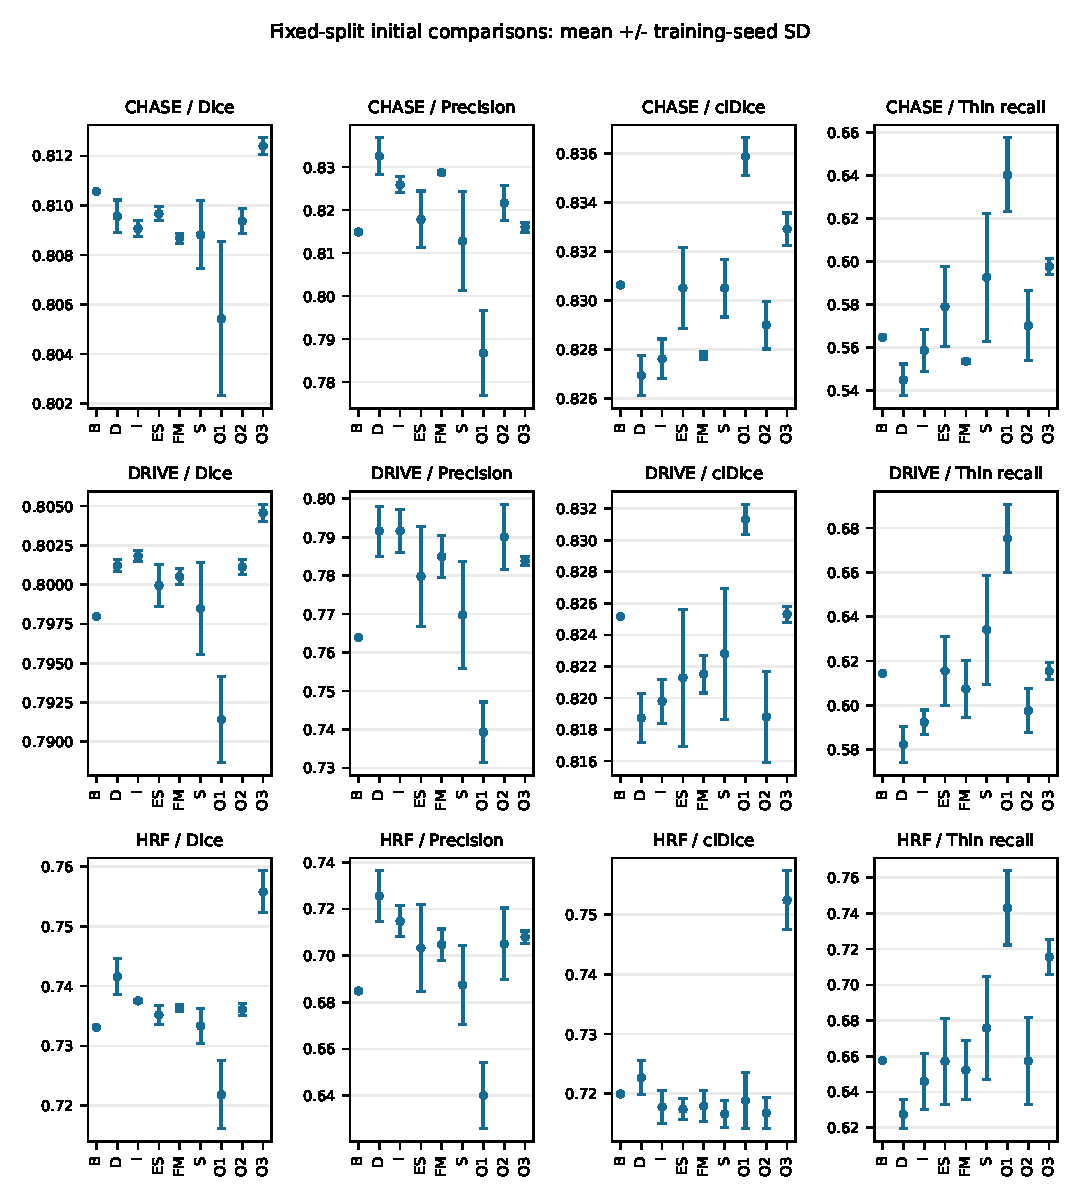
\includegraphics[width=\fulllength]{figures/initial_three_dataset_scores_2026-11-19_07-40-21.pdf}
\end{adjustwidth}\caption{Initial raw recipes on all three retained fixed cohorts. B: frozen baseline; D: Direct; I: endpoint-iterative; FM: full-target Flow; S: selective without gate; ES: ESFM; O1/O2/O3: the three initial recipes. Error bars show sample SD across five refiner-training seed means, conditional on the retained upstream models. The one frozen baseline has no training-seed SD. These bars are not population confidence intervals.}\label{fig:initial-comparison}\end{figure}
\Needspace{8\baselineskip}
\subsection{Sequential Flow and Matched Direct Results}
Tables~\ref{tab:followup-CHASE}--\ref{tab:followup-HRF} and Figure~\ref{fig:followup-comparison} summarize the sequential comparisons. Figure~\ref{fig:real-panels} displays identifier-selected examples from the saved outputs.



\begingroup\scriptsize\setlength{\tabcolsep}{3pt}\renewcommand{\arraystretch}{1.12}\setlength{\LTleft}{-\extralength}\setlength{\LTright}{0pt plus1fill}\setlength{\LTcapwidth}{\dimexpr 14.800cm+30pt\relax}\captionsetup[longtable]{margin=0pt,width=\LTcapwidth,singlelinecheck=false,justification=raggedright}\makeatletter\long\def\caption@LT@make#1{\LT@mcol\LT@cols{@{}l@{}}{\parbox[t]{\LTcapwidth}{#1}}}\makeatother
\begin{longtable}{@{}>{\raggedright\arraybackslash}p{4.1cm}>{\raggedright\arraybackslash}p{0.7cm}>{\raggedright\arraybackslash}p{2.5cm}>{\raggedright\arraybackslash}p{2.5cm}>{\raggedright\arraybackslash}p{2.5cm}>{\raggedright\arraybackslash}p{2.5cm}@{}}
\caption{CHASE: sequential follow-ups. Raw and validation-selected outputs are separate. Source and selection changes across phases prevent an additive causal interpretation.}\label{tab:followup-CHASE}\\
\toprule
Method / output & Seeds & Dice & Precision & clDice & Thin recall\\
\midrule\endfirsthead
\toprule
Method / output & Seeds & Dice & Precision & clDice & Thin recall\\
\midrule\endhead
\bottomrule\endfoot
F1 native FM  / blend & 5 & $0.810459\pm 0.000108$ & $0.815115\pm 0.002261$ & $0.830019\pm 0.000446$ & $0.574031\pm 0.012572$\\
F1 native FM  / raw & 5 & $0.809272\pm 0.000792$ & $0.821403\pm 0.005294$ & $0.829422\pm 0.001733$ & $0.566339\pm 0.019454$\\
F2 anchored FM  / raw & 5 & $0.812273\pm 0.000309$ & $0.816497\pm 0.001458$ & $0.832140\pm 0.000385$ & $0.596163\pm 0.005209$\\
F2 anchored FM  / selected & 5 & $0.812353\pm 0.000341$ & $0.816351\pm 0.001006$ & $0.832408\pm 0.000564$ & $0.596611\pm 0.004155$\\
F3 strict OOF  / raw & 5 & $0.812547\pm 0.000342$ & $0.814890\pm 0.002067$ & $0.832198\pm 0.000715$ & $0.599086\pm 0.005672$\\
F3 strict OOF  / selected & 5 & $0.812533\pm 0.000347$ & $0.815274\pm 0.001272$ & $0.832293\pm 0.000821$ & $0.598693\pm 0.005152$\\
F4 topology  / raw & 5 & $0.810757\pm 0.000338$ & $0.794838\pm 0.001792$ & $0.835038\pm 0.000620$ & $0.643479\pm 0.005001$\\
F4 topology  / selected & 5 & $0.812394\pm 0.000330$ & $0.814846\pm 0.001028$ & $0.833094\pm 0.000563$ & $0.601439\pm 0.004644$\\
F5 retained  / raw & 5 & $0.811260\pm 0.000637$ & $0.801428\pm 0.004690$ & $0.833994\pm 0.000968$ & $0.634950\pm 0.006587$\\
F5 retained  / selected & 5 & $0.812396\pm 0.000328$ & $0.815601\pm 0.001056$ & $0.833003\pm 0.000697$ & $0.598917\pm 0.003861$\\
F6 local acceptor direct / accepted & 5 & $0.812398\pm 0.000327$ & $0.815997\pm 0.001154$ & $0.832913\pm 0.000653$ & $0.597733\pm 0.003634$\\
F6 local acceptor direct / raw & 5 & $0.812389\pm 0.000327$ & $0.815896\pm 0.001143$ & $0.832933\pm 0.000678$ & $0.597973\pm 0.003645$\\
F6 local acceptor flow / accepted & 5 & $0.812398\pm 0.000327$ & $0.815997\pm 0.001154$ & $0.832913\pm 0.000653$ & $0.597733\pm 0.003634$\\
F6 local acceptor flow / raw & 5 & $0.812226\pm 0.000419$ & $0.815463\pm 0.001365$ & $0.832873\pm 0.000689$ & $0.598529\pm 0.004496$\\
F7 native rollout direct / selected & 5 & $0.812413\pm 0.000341$ & $0.813465\pm 0.002094$ & $0.832870\pm 0.000522$ & $0.605871\pm 0.008108$\\
F7 native rollout flow / selected & 5 & $0.812389\pm 0.000303$ & $0.812304\pm 0.002168$ & $0.832850\pm 0.000416$ & $0.609591\pm 0.004927$\\
F8 global context direct / selected & 5 & $0.812435\pm 0.000336$ & $0.814338\pm 0.001220$ & $0.833002\pm 0.000480$ & $0.603085\pm 0.006114$\\
F8 global context flow / selected & 5 & $0.812440\pm 0.000325$ & $0.813016\pm 0.002331$ & $0.833140\pm 0.000675$ & $0.607826\pm 0.007049$\\
\end{longtable}\endgroup

\begingroup\scriptsize\setlength{\tabcolsep}{3pt}\renewcommand{\arraystretch}{1.12}\setlength{\LTleft}{-\extralength}\setlength{\LTright}{0pt plus1fill}\setlength{\LTcapwidth}{\dimexpr 14.800cm+30pt\relax}\captionsetup[longtable]{margin=0pt,width=\LTcapwidth,singlelinecheck=false,justification=raggedright}\makeatletter\long\def\caption@LT@make#1{\LT@mcol\LT@cols{@{}l@{}}{\parbox[t]{\LTcapwidth}{#1}}}\makeatother
\begin{longtable}{@{}>{\raggedright\arraybackslash}p{4.1cm}>{\raggedright\arraybackslash}p{0.7cm}>{\raggedright\arraybackslash}p{2.5cm}>{\raggedright\arraybackslash}p{2.5cm}>{\raggedright\arraybackslash}p{2.5cm}>{\raggedright\arraybackslash}p{2.5cm}@{}}
\caption{DRIVE: sequential follow-ups. Raw and validation-selected outputs are separate. Source and selection changes across phases prevent an additive causal interpretation.}\label{tab:followup-DRIVE}\\
\toprule
Method / output & Seeds & Dice & Precision & clDice & Thin recall\\
\midrule\endfirsthead
\toprule
Method / output & Seeds & Dice & Precision & clDice & Thin recall\\
\midrule\endhead
\bottomrule\endfoot
F1 native FM  / blend & 5 & $0.800158\pm 0.000492$ & $0.782140\pm 0.005304$ & $0.821910\pm 0.001685$ & $0.603940\pm 0.003287$\\
F1 native FM  / raw & 5 & $0.800312\pm 0.000326$ & $0.783582\pm 0.003966$ & $0.821671\pm 0.001492$ & $0.602724\pm 0.003941$\\
F2 anchored FM  / raw & 5 & $0.804505\pm 0.000514$ & $0.784302\pm 0.001095$ & $0.824739\pm 0.000219$ & $0.614438\pm 0.002511$\\
F2 anchored FM  / selected & 5 & $0.804546\pm 0.000527$ & $0.784043\pm 0.001204$ & $0.825024\pm 0.000500$ & $0.615025\pm 0.003100$\\
F3 strict OOF  / raw & 5 & $0.804562\pm 0.000570$ & $0.784555\pm 0.000788$ & $0.823885\pm 0.000923$ & $0.607680\pm 0.004802$\\
F3 strict OOF  / selected & 5 & $0.804586\pm 0.000554$ & $0.783892\pm 0.001020$ & $0.824922\pm 0.000282$ & $0.613579\pm 0.003222$\\
F4 topology  / raw & 5 & $0.799637\pm 0.000715$ & $0.757393\pm 0.002116$ & $0.831738\pm 0.000088$ & $0.665920\pm 0.004729$\\
F4 topology  / selected & 5 & $0.804353\pm 0.000547$ & $0.782239\pm 0.001272$ & $0.825856\pm 0.000476$ & $0.619226\pm 0.004315$\\
F5 retained  / raw & 5 & $0.801188\pm 0.000877$ & $0.764720\pm 0.002468$ & $0.830469\pm 0.000211$ & $0.654199\pm 0.004218$\\
F5 retained  / selected & 5 & $0.804489\pm 0.000496$ & $0.783178\pm 0.001176$ & $0.825508\pm 0.000512$ & $0.616848\pm 0.003512$\\
F6 local acceptor direct / accepted & 5 & $0.804570\pm 0.000534$ & $0.783800\pm 0.001245$ & $0.825299\pm 0.000496$ & $0.615358\pm 0.003817$\\
F6 local acceptor direct / raw & 5 & $0.804331\pm 0.000866$ & $0.784369\pm 0.001002$ & $0.824778\pm 0.000795$ & $0.613161\pm 0.003823$\\
F6 local acceptor flow / accepted & 5 & $0.804570\pm 0.000534$ & $0.783800\pm 0.001245$ & $0.825299\pm 0.000496$ & $0.615358\pm 0.003817$\\
F6 local acceptor flow / raw & 5 & $0.804418\pm 0.000576$ & $0.783976\pm 0.001138$ & $0.825014\pm 0.000434$ & $0.614388\pm 0.003123$\\
F7 native rollout direct / raw & 5 & $0.804232\pm 0.000505$ & $0.775543\pm 0.005623$ & $0.827547\pm 0.001587$ & $0.642020\pm 0.019422$\\
F7 native rollout direct / selected & 5 & $0.804337\pm 0.000543$ & $0.777206\pm 0.006022$ & $0.827095\pm 0.001628$ & $0.636738\pm 0.020913$\\
F7 native rollout flow / raw & 5 & $0.803889\pm 0.000627$ & $0.771717\pm 0.001840$ & $0.828524\pm 0.000627$ & $0.654947\pm 0.007410$\\
F7 native rollout flow / selected & 5 & $0.804326\pm 0.000481$ & $0.776923\pm 0.004089$ & $0.827391\pm 0.001304$ & $0.638383\pm 0.015441$\\
F8 global context direct / raw & 5 & $0.804268\pm 0.000571$ & $0.776907\pm 0.002331$ & $0.827589\pm 0.000813$ & $0.636478\pm 0.007856$\\
F8 global context direct / selected & 5 & $0.804512\pm 0.000545$ & $0.780590\pm 0.002885$ & $0.826505\pm 0.001319$ & $0.625628\pm 0.010479$\\
F8 global context flow / raw & 5 & $0.803710\pm 0.000544$ & $0.773416\pm 0.004972$ & $0.828137\pm 0.001395$ & $0.649620\pm 0.017981$\\
F8 global context flow / selected & 5 & $0.804417\pm 0.000531$ & $0.779357\pm 0.003228$ & $0.827023\pm 0.001436$ & $0.630141\pm 0.010348$\\
\end{longtable}\endgroup

\begingroup\scriptsize\setlength{\tabcolsep}{3pt}\renewcommand{\arraystretch}{1.12}\setlength{\LTleft}{-\extralength}\setlength{\LTright}{0pt plus1fill}\setlength{\LTcapwidth}{\dimexpr 14.800cm+30pt\relax}\captionsetup[longtable]{margin=0pt,width=\LTcapwidth,singlelinecheck=false,justification=raggedright}\makeatletter\long\def\caption@LT@make#1{\LT@mcol\LT@cols{@{}l@{}}{\parbox[t]{\LTcapwidth}{#1}}}\makeatother
\begin{longtable}{@{}>{\raggedright\arraybackslash}p{4.1cm}>{\raggedright\arraybackslash}p{0.7cm}>{\raggedright\arraybackslash}p{2.5cm}>{\raggedright\arraybackslash}p{2.5cm}>{\raggedright\arraybackslash}p{2.5cm}>{\raggedright\arraybackslash}p{2.5cm}@{}}
\caption{HRF: sequential follow-ups. Raw and validation-selected outputs are separate. Source and selection changes across phases prevent an additive causal interpretation.}\label{tab:followup-HRF}\\
\toprule
Method / output & Seeds & Dice & Precision & clDice & Thin recall\\
\midrule\endfirsthead
\toprule
Method / output & Seeds & Dice & Precision & clDice & Thin recall\\
\midrule\endhead
\bottomrule\endfoot
F1 native FM  / blend & 5 & $0.739803\pm 0.004651$ & $0.691354\pm 0.012246$ & $0.734197\pm 0.013081$ & $0.682366\pm 0.030163$\\
F1 native FM  / raw & 5 & $0.738338\pm 0.005571$ & $0.685759\pm 0.021775$ & $0.739325\pm 0.018209$ & $0.691623\pm 0.039388$\\
F2 anchored FM  / raw & 5 & $0.755802\pm 0.003672$ & $0.706392\pm 0.002747$ & $0.752391\pm 0.005495$ & $0.722289\pm 0.013745$\\
F2 anchored FM  / selected & 5 & $0.756015\pm 0.003499$ & $0.706719\pm 0.002122$ & $0.752740\pm 0.005078$ & $0.721587\pm 0.012604$\\
F3 strict OOF  / raw & 5 & $0.755604\pm 0.003383$ & $0.704488\pm 0.002754$ & $0.752335\pm 0.004427$ & $0.725052\pm 0.016226$\\
F3 strict OOF  / selected & 5 & $0.755731\pm 0.003451$ & $0.705228\pm 0.003624$ & $0.752557\pm 0.004558$ & $0.723038\pm 0.016180$\\
F4 topology  / raw & 5 & $0.749517\pm 0.003276$ & $0.675446\pm 0.003068$ & $0.752694\pm 0.003831$ & $0.765680\pm 0.011530$\\
F4 topology  / selected & 5 & $0.755753\pm 0.003517$ & $0.707885\pm 0.002634$ & $0.752433\pm 0.004938$ & $0.715623\pm 0.009706$\\
F5 retained  / raw & 5 & $0.752489\pm 0.003230$ & $0.685349\pm 0.003385$ & $0.752997\pm 0.003906$ & $0.755631\pm 0.011322$\\
F5 retained  / selected & 5 & $0.755702\pm 0.003534$ & $0.705833\pm 0.002652$ & $0.752716\pm 0.004947$ & $0.720195\pm 0.010022$\\
F6 local acceptor direct / accepted & 5 & $0.755753\pm 0.003517$ & $0.707885\pm 0.002634$ & $0.752433\pm 0.004938$ & $0.715623\pm 0.009706$\\
F6 local acceptor direct / raw & 5 & $0.755916\pm 0.004143$ & $0.709746\pm 0.005247$ & $0.752474\pm 0.005165$ & $0.715356\pm 0.009598$\\
F6 local acceptor flow / accepted & 5 & $0.755753\pm 0.003517$ & $0.707885\pm 0.002634$ & $0.752433\pm 0.004938$ & $0.715623\pm 0.009706$\\
F6 local acceptor flow / raw & 5 & $0.756130\pm 0.003952$ & $0.709743\pm 0.004657$ & $0.752449\pm 0.005012$ & $0.715342\pm 0.009553$\\
F7 native rollout direct / raw & 5 & $0.756777\pm 0.002453$ & $0.686725\pm 0.002274$ & $0.755558\pm 0.004025$ & $0.780351\pm 0.010712$\\
F7 native rollout direct / selected & 5 & $0.756626\pm 0.002557$ & $0.686385\pm 0.002215$ & $0.755479\pm 0.003864$ & $0.781031\pm 0.009695$\\
F7 native rollout flow / raw & 5 & $0.756951\pm 0.002440$ & $0.686780\pm 0.002511$ & $0.757404\pm 0.003461$ & $0.780101\pm 0.007332$\\
F7 native rollout flow / selected & 5 & $0.756768\pm 0.002332$ & $0.685985\pm 0.002467$ & $0.757095\pm 0.003603$ & $0.781960\pm 0.009639$\\
F8 global context direct / raw & 5 & $0.757375\pm 0.002836$ & $0.690095\pm 0.006707$ & $0.756486\pm 0.003995$ & $0.772965\pm 0.011216$\\
F8 global context direct / selected & 5 & $0.756512\pm 0.002438$ & $0.685940\pm 0.002061$ & $0.755169\pm 0.003784$ & $0.781745\pm 0.009941$\\
F8 global context flow / raw & 5 & $0.756701\pm 0.002324$ & $0.686489\pm 0.002634$ & $0.756786\pm 0.002934$ & $0.781089\pm 0.009541$\\
F8 global context flow / selected & 5 & $0.756718\pm 0.002318$ & $0.686536\pm 0.002666$ & $0.756769\pm 0.002919$ & $0.781389\pm 0.008995$\\
\end{longtable}\endgroup

\begin{figure}[htbp]\begin{adjustwidth}{-\extralength}{0cm}\centering
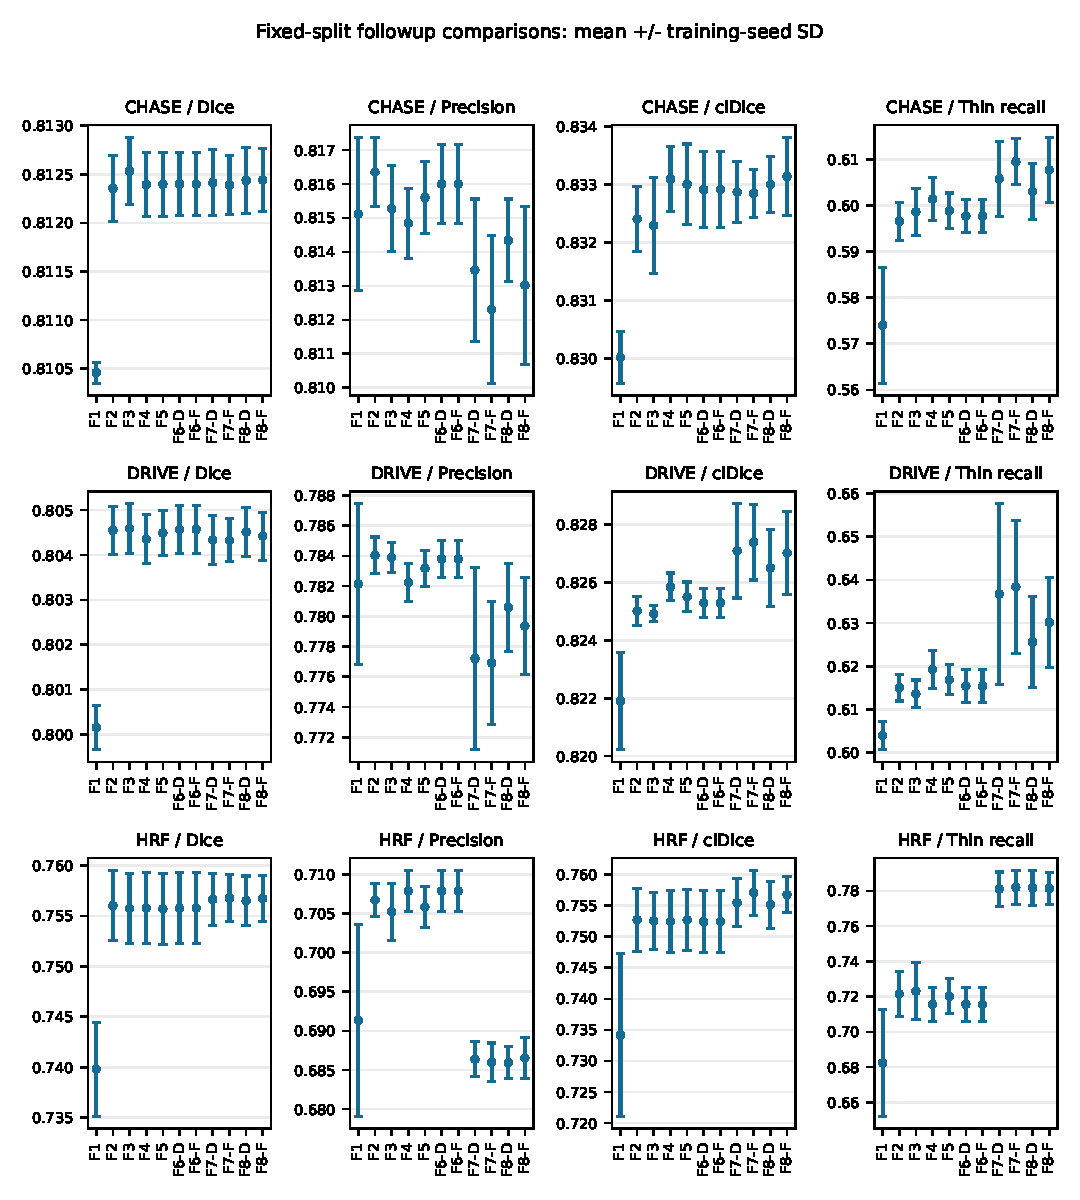
\includegraphics[width=\fulllength]{figures/followup_three_dataset_scores_2026-11-19_07-40-21.pdf}
\end{adjustwidth}\caption{Validation-selected fixed-split outputs. F1--F8 follow the method definitions; suffix F denotes Flow and D denotes its matched direct control. Parameter matching is phase-specific; field-evaluation and candidate-grid counts differ. Selection includes exact anchor fallback, and repeated validation use is exploratory. These phases are not an additive learning curve.}\label{fig:followup-comparison}\end{figure}

\begin{figure}[htbp]\begin{adjustwidth}{-\extralength}{0cm}\centering
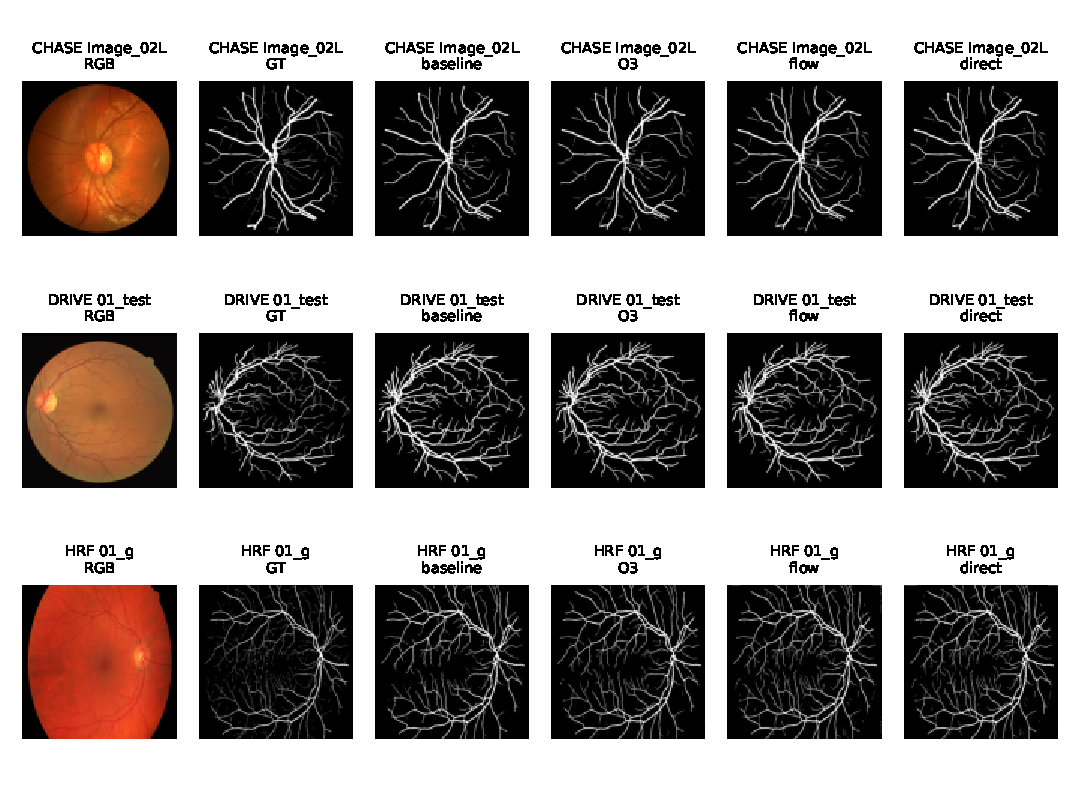
\includegraphics[width=\fulllength]{figures/prespecified_real_prediction_panels_2026-11-19_07-40-21.pdf}
\end{adjustwidth}\caption{Real saved seed 42 predictions for the first image identifier in each original test split. The cases are selected by identifier before comparing scores. Columns show the original RGB image, GT, baseline, O3 and the validation-selected whole-image-context Flow and direct outputs. Identical panels are retained when the system selects identity; no generated prediction or manually repaired vessel is substituted.}\label{fig:real-panels}\end{figure}
\Needspace{8\baselineskip}
\subsection{Fresh Outer-CV Comparison}
Table~\ref{tab:fresh-cv} and Figure~\ref{fig:fresh-cv-changes} report the fresh held-out comparisons. Table~\ref{tab:calibrated-cv} and Figure~\ref{fig:calibrated-cv-changes} retain the separate, conditional calibration extension.



\begingroup\scriptsize\setlength{\tabcolsep}{3pt}\renewcommand{\arraystretch}{1.12}\setlength{\LTleft}{-\extralength}\setlength{\LTright}{0pt plus1fill}\setlength{\LTcapwidth}{\dimexpr 14.700cm+36pt\relax}\captionsetup[longtable]{margin=0pt,width=\LTcapwidth,singlelinecheck=false,justification=raggedright}\makeatletter\long\def\caption@LT@make#1{\LT@mcol\LT@cols{@{}l@{}}{\parbox[t]{\LTcapwidth}{#1}}}\makeatother
\begin{longtable}{@{}>{\raggedright\arraybackslash}p{1.3cm}>{\raggedright\arraybackslash}p{2.4cm}>{\raggedright\arraybackslash}p{1.0cm}>{\raggedright\arraybackslash}p{2.5cm}>{\raggedright\arraybackslash}p{2.5cm}>{\raggedright\arraybackslash}p{2.5cm}>{\raggedright\arraybackslash}p{2.5cm}@{}}
\caption{Fresh outer-CV scores. CHASE uses 28 images, DRIVE 40 and HRF 45. CHASE retains selected CV outputs only; raw scores are reported where archived on DRIVE/HRF. SD describes correction-stage seed variation conditional on shared fresh upstream models; it is not SD over five complete pipelines.}\label{tab:fresh-cv}\\
\toprule
Dataset & Method / output & Images & Dice & Precision & clDice & Thin recall\\
\midrule\endfirsthead
\toprule
Dataset & Method / output & Images & Dice & Precision & clDice & Thin recall\\
\midrule\endhead
\bottomrule\endfoot
CHASE & direct / selected & 28 & $0.815807\pm 0.000000$ & $0.797007\pm 0.000000$ & $0.830832\pm 0.000000$ & $0.600233\pm 0.000000$\\
CHASE & flow / selected & 28 & $0.815807\pm 0.000000$ & $0.797007\pm 0.000000$ & $0.830832\pm 0.000000$ & $0.600233\pm 0.000000$\\
CHASE & baseline / anchor & 28 & $0.814358$ & $0.796506$ & $0.829747$ & $0.576182$\\
CHASE & O3 / anchor & 28 & $0.815807$ & $0.797007$ & $0.830832$ & $0.600233$\\
DRIVE & direct / raw & 40 & $0.800369\pm 0.000318$ & $0.793684\pm 0.003169$ & $0.813241\pm 0.000656$ & $0.589714\pm 0.010288$\\
DRIVE & direct / selected & 40 & $0.800042\pm 0.000000$ & $0.802428\pm 0.000000$ & $0.810148\pm 0.000000$ & $0.560238\pm 0.000000$\\
DRIVE & flow / raw & 40 & $0.800155\pm 0.000521$ & $0.793806\pm 0.003029$ & $0.812524\pm 0.000251$ & $0.589917\pm 0.009207$\\
DRIVE & flow / selected & 40 & $0.800042\pm 0.000000$ & $0.802428\pm 0.000000$ & $0.810148\pm 0.000000$ & $0.560238\pm 0.000000$\\
DRIVE & baseline / anchor & 40 & $0.796438$ & $0.800118$ & $0.807250$ & $0.542323$\\
DRIVE & O3 / anchor & 40 & $0.800042$ & $0.802428$ & $0.810148$ & $0.560238$\\
HRF & direct / raw & 45 & $0.762058\pm 0.000155$ & $0.708537\pm 0.000399$ & $0.762392\pm 0.000391$ & $0.732639\pm 0.002067$\\
HRF & direct / selected & 45 & $0.759100\pm 0.000000$ & $0.721265\pm 0.000000$ & $0.754823\pm 0.000000$ & $0.684556\pm 0.000000$\\
HRF & flow / raw & 45 & $0.761797\pm 0.000309$ & $0.708218\pm 0.000953$ & $0.762372\pm 0.000690$ & $0.732914\pm 0.002034$\\
HRF & flow / selected & 45 & $0.759100\pm 0.000000$ & $0.721265\pm 0.000000$ & $0.754823\pm 0.000000$ & $0.684556\pm 0.000000$\\
HRF & baseline / anchor & 45 & $0.741575$ & $0.705310$ & $0.727467$ & $0.635815$\\
HRF & O3 / anchor & 45 & $0.759100$ & $0.721265$ & $0.754823$ & $0.684556$\\
\end{longtable}\endgroup

\begin{figure}[htbp]\begin{adjustwidth}{-\extralength}{0cm}\centering
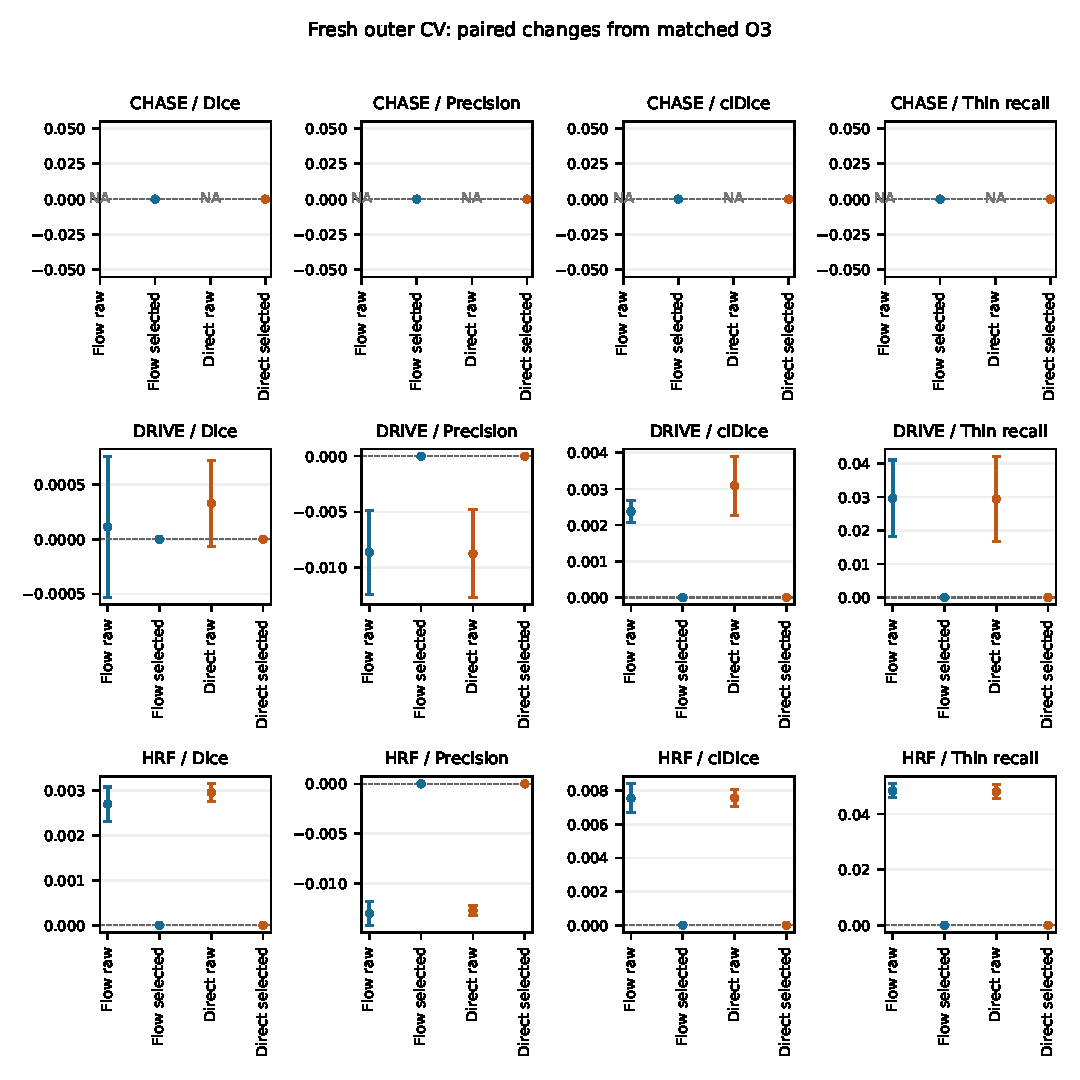
\includegraphics[width=\fulllength]{figures/fresh_CV_paired_changes_2026-11-19_07-40-21.pdf}
\end{adjustwidth}\caption{Fresh outer-CV changes relative to the matched O3 sources. Points are means over five correction seeds; bars show pointwise seed-level paired $t$ 95\% confidence intervals, where defined. NA marks the unarchived CHASE raw CV outputs; no score is imputed. Both arms share the freshly trained upstream models within each fold. Raw denotes the validation-ranked learned candidate without the preservation gate; selected outputs include exact identity. The intervals are conditional on the retained cohort and shared upstream fits, and do not quantify full-pipeline or prospective clinical uncertainty.}\label{fig:fresh-cv-changes}\end{figure}

\begingroup\scriptsize\setlength{\tabcolsep}{3pt}\renewcommand{\arraystretch}{1.12}\setlength{\LTleft}{-\extralength}\setlength{\LTright}{0pt plus1fill}\setlength{\LTcapwidth}{\dimexpr 14.700cm+36pt\relax}\captionsetup[longtable]{margin=0pt,width=\LTcapwidth,singlelinecheck=false,justification=raggedright}\makeatletter\long\def\caption@LT@make#1{\LT@mcol\LT@cols{@{}l@{}}{\parbox[t]{\LTcapwidth}{#1}}}\makeatother
\begin{longtable}{@{}>{\raggedright\arraybackslash}p{1.3cm}>{\raggedright\arraybackslash}p{2.4cm}>{\raggedright\arraybackslash}p{1.0cm}>{\raggedright\arraybackslash}p{2.5cm}>{\raggedright\arraybackslash}p{2.5cm}>{\raggedright\arraybackslash}p{2.5cm}>{\raggedright\arraybackslash}p{2.5cm}@{}}
\caption{Conditional calibration extension on datasets whose single-seed validation pilot passes. The calibrated O3 baseline is separate from the original 0.5 baseline. No unexecuted CHASE calibration-test result is inferred.}\label{tab:calibrated-cv}\\
\toprule
Data & Output & Images & Dice & Precision & clDice & Thin recall\\
\midrule\endfirsthead
\toprule
Data & Output & Images & Dice & Precision & clDice & Thin recall\\
\midrule\endhead
\bottomrule\endfoot
DRIVE & baseline / anchor & 40 & $0.796438$ & $0.800118$ & $0.807250$ & $0.542323$\\
DRIVE & O3 / anchor & 40 & $0.800042$ & $0.802428$ & $0.810148$ & $0.560238$\\
DRIVE & direct / selected & 40 & $0.800444\pm 0.000185$ & $0.802870\pm 0.000730$ & $0.810430\pm 0.000458$ & $0.574897\pm 0.003055$\\
DRIVE & flow / selected & 40 & $0.800326\pm 0.000124$ & $0.802582\pm 0.000194$ & $0.810430\pm 0.000271$ & $0.573947\pm 0.002677$\\
HRF & baseline / anchor & 45 & $0.741575$ & $0.705310$ & $0.727467$ & $0.635815$\\
HRF & O3 / anchor & 45 & $0.759100$ & $0.721265$ & $0.754823$ & $0.684556$\\
HRF & direct / selected & 45 & $0.764407\pm 0.000282$ & $0.721431\pm 0.000090$ & $0.761797\pm 0.000369$ & $0.717834\pm 0.001961$\\
HRF & flow / selected & 45 & $0.763971\pm 0.000255$ & $0.721282\pm 0.000138$ & $0.761343\pm 0.000512$ & $0.717721\pm 0.001443$\\
\end{longtable}\endgroup

\begin{figure}[htbp]\begin{adjustwidth}{-\extralength}{0cm}\centering
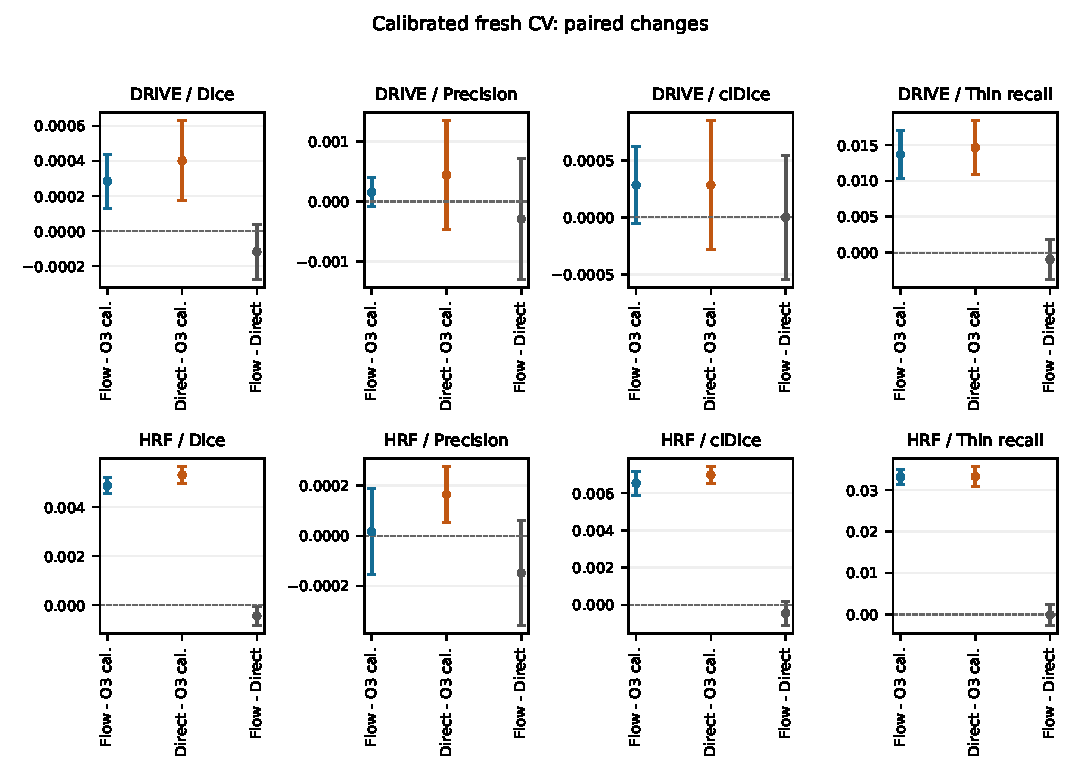
\includegraphics[width=\fulllength]{figures/calibrated_CV_paired_changes_2026-11-19_07-40-21.pdf}
\end{adjustwidth}\caption{Conditional calibrated outer-CV contrasts. Points are five-seed mean differences and bars are pointwise paired $t$ 95\% intervals. Each fold calibrates O3 separately on validation data. The gray contrast compares Flow directly with its matched direct control. These intervals describe correction-seed variation conditional on the shared source fits and retained cohort. The plotted comparisons do not establish a general Flow-specific advantage.}\label{fig:calibrated-cv-changes}\end{figure}
\Needspace{8\baselineskip}
\subsection{Paired Contrasts and Diagnostic Scope}
Table~\ref{tab:paired-all} contains the selected-output paired contrasts. Table~\ref{tab:geometry-pilots} reports the single-fit geometry pilots; Tables~\ref{tab:retention-vs-prior} and~\ref{tab:warm-reuse} separate F5 retention from warm-field reuse. Table~\ref{tab:frunet-pilots} lists the FR-UNet validation fits.


The full paired tables include both seed-based and crossed-bootstrap intervals, unadjusted tests, Holm families and identity cases. Five-seed exact signed-rank tests have coarse resolution; a nonsignificant result is not an equivalence claim. The encoded-flow and geometry pilots remain single-training diagnostics. FR-UNet has three validation learning-rate pilots per dataset; no five-seed FR-UNet test study is inferred from them. The newly completed SegFlow HRF comparison uses five previously fitted checkpoints. Threshold, precision-guard and connection/oracle diagnostics are validation-only and are not pooled with test efficacy.

\begingroup\scriptsize\setlength{\tabcolsep}{3pt}\renewcommand{\arraystretch}{1.12}\setlength{\LTleft}{-\extralength}\setlength{\LTright}{0pt plus1fill}\setlength{\LTcapwidth}{\dimexpr 15.100cm+30pt\relax}\captionsetup[longtable]{margin=0pt,width=\LTcapwidth,singlelinecheck=false,justification=raggedright}\makeatletter\long\def\caption@LT@make#1{\LT@mcol\LT@cols{@{}l@{}}{\parbox[t]{\LTcapwidth}{#1}}}\makeatother
\begin{longtable}{@{}>{\raggedright\arraybackslash}p{1.1cm}>{\raggedright\arraybackslash}p{4.0cm}>{\raggedright\arraybackslash}p{2.5cm}>{\raggedright\arraybackslash}p{2.5cm}>{\raggedright\arraybackslash}p{2.5cm}>{\raggedright\arraybackslash}p{2.5cm}@{}}
\caption{Single-fit geometry pilots: validation means only. The selected and raw validation-ranked candidates are distinct; no SD, five-seed confirmation or new test score is implied.}\label{tab:geometry-pilots}\\
\toprule
Data & Candidate & Dice & Precision & clDice & Thin recall\\
\midrule\endfirsthead
\toprule
Data & Candidate & Dice & Precision & clDice & Thin recall\\
\midrule\endhead
\bottomrule\endfoot
CHASE & O3 validation & 0.831430 & 0.838153 & 0.839091 & 0.608629\\
CHASE & Selected geometry pilot & 0.831430 & 0.838153 & 0.839091 & 0.608629\\
CHASE & Raw validation-ranked candidate & 0.831150 & 0.839179 & 0.838933 & 0.626572\\
DRIVE & O3 validation & 0.767930 & 0.756611 & 0.782051 & 0.564246\\
DRIVE & Selected geometry pilot & 0.767930 & 0.756611 & 0.782051 & 0.564246\\
DRIVE & Raw validation-ranked candidate & 0.767937 & 0.756472 & 0.782066 & 0.567299\\
HRF & O3 validation & 0.762266 & 0.740560 & 0.756681 & 0.658573\\
HRF & Selected geometry pilot & 0.764843 & 0.742265 & 0.758635 & 0.681610\\
HRF & Raw validation-ranked candidate & 0.765280 & 0.743547 & 0.760102 & 0.678844\\
\end{longtable}\endgroup

\begingroup\scriptsize\setlength{\tabcolsep}{3pt}\renewcommand{\arraystretch}{1.12}\setlength{\LTleft}{-\extralength}\setlength{\LTright}{0pt plus1fill}\setlength{\LTcapwidth}{\dimexpr 14.000cm+30pt\relax}\captionsetup[longtable]{margin=0pt,width=\LTcapwidth,singlelinecheck=false,justification=raggedright}\makeatletter\long\def\caption@LT@make#1{\LT@mcol\LT@cols{@{}l@{}}{\parbox[t]{\LTcapwidth}{#1}}}\makeatother
\begin{longtable}{@{}>{\raggedright\arraybackslash}p{1.2cm}>{\raggedright\arraybackslash}p{3.0cm}>{\raggedright\arraybackslash}p{2.0cm}>{\raggedright\arraybackslash}p{3.6cm}>{\raggedright\arraybackslash}p{2.2cm}>{\raggedright\arraybackslash}p{2.0cm}@{}}
\caption{F5 selected minus preceding F4 selected on matched test images and training seeds. Validation retention does not imply test retention. CI is the seed-level t interval; exact signed-rank p is unadjusted. Multiple recipe factors differ, so this is a system comparison.}\label{tab:retention-vs-prior}\\
\toprule
Data & Outcome & Mean change & 95\% CI & Holm t p & Exact W p\\
\midrule\endfirsthead
\toprule
Data & Outcome & Mean change & 95\% CI & Holm t p & Exact W p\\
\midrule\endhead
\bottomrule\endfoot
HRF & Dice & -0.000052 & $[-0.000116,0.000013]$ & 0.659818 & 0.187500\\
HRF & Precision & -0.002052 & $[-0.002109,-0.001996]$ & $<10^{-6}$ & 0.062500\\
HRF & clDice & 0.000283 & $[0.000162,0.000404]$ & 0.028835 & 0.062500\\
HRF & Thin recall & 0.004572 & $[0.003979,0.005166]$ & 0.000311 & 0.062500\\
CHASE & Dice & \ensuremath{2.192\times10^{-6}} & $[-0.000021,0.000025]$ & 0.862285 & 0.875000\\
CHASE & Precision & 0.000755 & $[-0.000114,0.001623]$ & 0.659818 & 0.125000\\
CHASE & clDice & -0.000091 & $[-0.000357,0.000174]$ & 0.862285 & 0.625000\\
CHASE & Thin recall & -0.002522 & $[-0.005544,0.000501]$ & 0.659818 & 0.250000\\
DRIVE & Dice & 0.000137 & $[-0.000078,0.000351]$ & 0.862285 & 0.187500\\
DRIVE & Precision & 0.000939 & $[-0.000529,0.002407]$ & 0.862285 & 0.187500\\
DRIVE & clDice & -0.000347 & $[-0.000915,0.000221]$ & 0.862285 & 0.187500\\
DRIVE & Thin recall & -0.002378 & $[-0.006016,0.001260]$ & 0.862285 & 0.187500\\
\end{longtable}\endgroup

\begingroup\scriptsize\setlength{\tabcolsep}{3pt}\renewcommand{\arraystretch}{1.12}\setlength{\LTleft}{-\extralength}\setlength{\LTright}{0pt plus1fill}\setlength{\LTcapwidth}{\dimexpr 14.200cm+24pt\relax}\captionsetup[longtable]{margin=0pt,width=\LTcapwidth,singlelinecheck=false,justification=raggedright}\makeatletter\long\def\caption@LT@make#1{\LT@mcol\LT@cols{@{}l@{}}{\parbox[t]{\LTcapwidth}{#1}}}\makeatother
\begin{longtable}{@{}>{\raggedright\arraybackslash}p{1.5cm}>{\raggedright\arraybackslash}p{3.0cm}>{\raggedright\arraybackslash}p{2.5cm}>{\raggedright\arraybackslash}p{4.2cm}>{\raggedright\arraybackslash}p{3.0cm}@{}}
\caption{F5 initialization and reuse accounting across five final seeds. An epoch-zero warm choice uses an already retained F4 field; it is not credited as a newly learned F5 improvement. Zero strength instead returns O3.}\label{tab:warm-reuse}\\
\toprule
Data & Selected family & Warm starts & Nonzero epoch-zero reuse & Zero-strength choices\\
\midrule\endfirsthead
\toprule
Data & Selected family & Warm starts & Nonzero epoch-zero reuse & Zero-strength choices\\
\midrule\endhead
\bottomrule\endfoot
CHASE & warm & 5 & 0 & 3\\
DRIVE & signed & 0 & 0 & 3\\
HRF & signed & 0 & 0 & 0\\
\end{longtable}\endgroup

\begingroup\scriptsize\setlength{\tabcolsep}{3pt}\renewcommand{\arraystretch}{1.12}\setlength{\LTleft}{-\extralength}\setlength{\LTright}{0pt plus1fill}\setlength{\LTcapwidth}{\dimexpr 11.000cm+18pt\relax}\captionsetup[longtable]{margin=0pt,width=\LTcapwidth,singlelinecheck=false,justification=raggedright}\makeatletter\long\def\caption@LT@make#1{\LT@mcol\LT@cols{@{}l@{}}{\parbox[t]{\LTcapwidth}{#1}}}\makeatother
\begin{longtable}{@{}>{\raggedright\arraybackslash}p{2.0cm}>{\raggedright\arraybackslash}p{3.0cm}>{\raggedright\arraybackslash}p{3.0cm}>{\raggedright\arraybackslash}p{3.0cm}@{}}
\caption{FR-UNet validation-learning-rate pilots. Each row is one seed 91011 fit; these are tuning records, not three independent training seeds or a test benchmark.}\label{tab:frunet-pilots}\\
\toprule
Data & Learning rate & Selected epoch & Validation Dice\\
\midrule\endfirsthead
\toprule
Data & Learning rate & Selected epoch & Validation Dice\\
\midrule\endhead
\bottomrule\endfoot
CHASE & 0.0001 & 100 & 0.754927\\
CHASE & 0.0003 & 120 & 0.788512\\
CHASE & 1e-05 & 90 & 0.644561\\
DRIVE & 0.0001 & 100 & 0.724322\\
DRIVE & 0.0003 & 110 & 0.750822\\
DRIVE & 1e-05 & 90 & 0.618239\\
HRF & 0.0001 & 120 & 0.679747\\
HRF & 0.0003 & 120 & 0.712074\\
HRF & 1e-05 & 90 & 0.621436\\
\end{longtable}\endgroup
\Needspace{8\baselineskip}
\subsection{Validation Diagnostics and Rejected Candidates}
Tables~\ref{tab:encoded-diagnostics} and~\ref{tab:solver-diagnostics} retain the representation and solver probes. Tables~\ref{tab:boundary-diagnosis} and~\ref{tab:precision-reselection} report the boundary and precision screens. Calibration, connection and strength/bias diagnostics appear in Tables~\ref{tab:calibration-validation}--\ref{tab:bias-probe}.



\begingroup\scriptsize\setlength{\tabcolsep}{3pt}\renewcommand{\arraystretch}{1.12}\setlength{\LTleft}{-\extralength}\setlength{\LTright}{0pt plus1fill}\setlength{\LTcapwidth}{\dimexpr 14.000cm+12pt\relax}\captionsetup[longtable]{margin=0pt,width=\LTcapwidth,singlelinecheck=false,justification=raggedright}\makeatletter\long\def\caption@LT@make#1{\LT@mcol\LT@cols{@{}l@{}}{\parbox[t]{\LTcapwidth}{#1}}}\makeatother
\begin{longtable}{@{}>{\raggedright\arraybackslash}p{1.5cm}>{\raggedright\arraybackslash}p{9.0cm}>{\raggedright\arraybackslash}p{3.5cm}@{}}
\caption{Encoded-representation diagnostics: validation Dice only, one trained model. AE(GT) is a representation probe, not an attainable-performance upper bound. Euler 100 and zero-noise outputs are diagnostic replays, not replacement test models.}\label{tab:encoded-diagnostics}\\
\toprule
Data & Probe & Validation Dice\\
\midrule\endfirsthead
\toprule
Data & Probe & Validation Dice\\
\midrule\endhead
\bottomrule\endfoot
CHASE & ae\_coarse\_reconstruction & 0.766036\\
CHASE & ae\_gt\_reconstruction\_diagnostic\_not\_upper\_bound & 0.807393\\
CHASE & baseline & 0.828927\\
CHASE & euler100\_same\_noise & 0.759340\\
CHASE & euler20\_no\_noise & 0.759162\\
CHASE & euler20\_reproduced\_exactly & 0.762326\\
DRIVE & ae\_coarse\_reconstruction & 0.761825\\
DRIVE & ae\_gt\_reconstruction\_diagnostic\_not\_upper\_bound & 0.971507\\
DRIVE & baseline & 0.762614\\
DRIVE & euler100\_same\_noise & 0.729224\\
DRIVE & euler20\_no\_noise & 0.725781\\
DRIVE & euler20\_reproduced\_exactly & 0.732998\\
HRF & ae\_coarse\_reconstruction & 0.671280\\
HRF & ae\_gt\_reconstruction\_diagnostic\_not\_upper\_bound & 0.722040\\
HRF & baseline & 0.744959\\
HRF & euler100\_same\_noise & 0.676660\\
HRF & euler20\_no\_noise & 0.681329\\
HRF & euler20\_reproduced\_exactly & 0.678555\\
\end{longtable}\endgroup

\begingroup\scriptsize\setlength{\tabcolsep}{3pt}\renewcommand{\arraystretch}{1.12}\setlength{\LTleft}{-\extralength}\setlength{\LTright}{0pt plus1fill}\setlength{\LTcapwidth}{\dimexpr 10.000cm+12pt\relax}\captionsetup[longtable]{margin=0pt,width=\LTcapwidth,singlelinecheck=false,justification=raggedright}\makeatletter\long\def\caption@LT@make#1{\LT@mcol\LT@cols{@{}l@{}}{\parbox[t]{\LTcapwidth}{#1}}}\makeatother
\begin{longtable}{@{}>{\raggedright\arraybackslash}p{2.0cm}>{\raggedright\arraybackslash}p{4.0cm}>{\raggedright\arraybackslash}p{4.0cm}@{}}
\caption{Native F1 solver probe, validation only, seed 42. The training and deployed solver recipe is unchanged by this diagnostic.}\label{tab:solver-diagnostics}\\
\toprule
Data & Euler updates & Validation Dice\\
\midrule\endfirsthead
\toprule
Data & Euler updates & Validation Dice\\
\midrule\endhead
\bottomrule\endfoot
CHASE & 1 & 0.828207\\
CHASE & 2 & 0.828186\\
CHASE & 4 & 0.828216\\
CHASE & 8 & 0.828223\\
DRIVE & 1 & 0.764309\\
DRIVE & 2 & 0.764405\\
DRIVE & 4 & 0.764383\\
DRIVE & 8 & 0.764414\\
HRF & 1 & 0.746852\\
HRF & 2 & 0.747635\\
HRF & 4 & 0.747740\\
HRF & 8 & 0.747757\\
\end{longtable}\endgroup

\begingroup\scriptsize\setlength{\tabcolsep}{3pt}\renewcommand{\arraystretch}{1.12}\setlength{\LTleft}{-\extralength}\setlength{\LTright}{0pt plus1fill}\setlength{\LTcapwidth}{\dimexpr 12.000cm+18pt\relax}\captionsetup[longtable]{margin=0pt,width=\LTcapwidth,singlelinecheck=false,justification=raggedright}\makeatletter\long\def\caption@LT@make#1{\LT@mcol\LT@cols{@{}l@{}}{\parbox[t]{\LTcapwidth}{#1}}}\makeatother
\begin{longtable}{@{}>{\raggedright\arraybackslash}p{1.5cm}>{\raggedright\arraybackslash}p{3.0cm}>{\raggedright\arraybackslash}p{4.5cm}>{\raggedright\arraybackslash}p{3.0cm}@{}}
\caption{Validation added-false-positive diagnosis of the preceding seed 42 rollout. Boundary adjacency means distance at most 1.5 evaluation pixels from O3. A fraction is unavailable when no FP is added. Counts are restricted to the retained FOV; they do not establish anatomical false bridges. The geometry pilot extension is run regardless of whether its original CHASE adjacency heuristic holds.}\label{tab:boundary-diagnosis}\\
\toprule
Data & Added FP & Boundary-adjacent FP & Fraction\\
\midrule\endfirsthead
\toprule
Data & Added FP & Boundary-adjacent FP & Fraction\\
\midrule\endhead
\bottomrule\endfoot
CHASE & 865 & 746 & 0.862428\\
DRIVE & 822 & 736 & 0.895377\\
HRF & 4668 & 2707 & 0.579906\\
\end{longtable}\endgroup

\begingroup\scriptsize\setlength{\tabcolsep}{3pt}\renewcommand{\arraystretch}{1.12}\setlength{\LTleft}{-\extralength}\setlength{\LTright}{0pt plus1fill}\setlength{\LTcapwidth}{\dimexpr 12.000cm+18pt\relax}\captionsetup[longtable]{margin=0pt,width=\LTcapwidth,singlelinecheck=false,justification=raggedright}\makeatletter\long\def\caption@LT@make#1{\LT@mcol\LT@cols{@{}l@{}}{\parbox[t]{\LTcapwidth}{#1}}}\makeatother
\begin{longtable}{@{}>{\raggedright\arraybackslash}p{1.5cm}>{\raggedright\arraybackslash}p{2.5cm}>{\raggedright\arraybackslash}p{4.0cm}>{\raggedright\arraybackslash}p{4.0cm}@{}}
\caption{Retrospective four-metric precision guard on the fixed-cohort F8 validation grids. Each mode has five stored training seeds. Identity is an explicit rejection outcome, not a learned gain.}\label{tab:precision-reselection}\\
\toprule
Data & Arm & Nonzero choices & Identity choices\\
\midrule\endfirsthead
\toprule
Data & Arm & Nonzero choices & Identity choices\\
\midrule\endhead
\bottomrule\endfoot
CHASE & flow & 0 & 5\\
CHASE & direct & 0 & 5\\
DRIVE & flow & 0 & 5\\
DRIVE & direct & 0 & 5\\
HRF & flow & 0 & 5\\
HRF & direct & 0 & 5\\
\end{longtable}\endgroup

\begingroup\scriptsize\setlength{\tabcolsep}{3pt}\renewcommand{\arraystretch}{1.12}\setlength{\LTleft}{-\extralength}\setlength{\LTright}{0pt plus1fill}\setlength{\LTcapwidth}{\dimexpr 13.900cm+42pt\relax}\captionsetup[longtable]{margin=0pt,width=\LTcapwidth,singlelinecheck=false,justification=raggedright}\makeatletter\long\def\caption@LT@make#1{\LT@mcol\LT@cols{@{}l@{}}{\parbox[t]{\LTcapwidth}{#1}}}\makeatother
\begin{longtable}{@{}>{\raggedright\arraybackslash}p{1.0cm}>{\raggedright\arraybackslash}p{2.8cm}>{\raggedright\arraybackslash}p{0.8cm}>{\raggedright\arraybackslash}p{2.1cm}>{\raggedright\arraybackslash}p{2.1cm}>{\raggedright\arraybackslash}p{2.1cm}>{\raggedright\arraybackslash}p{2.1cm}>{\raggedright\arraybackslash}p{0.9cm}@{}}
\caption{Threshold-calibration pilot: equal-fold validation means for seed 42, not test scores. NZ counts the three fold-specific nonzero Flow/direct corrections. The same aggregate four-metric Flow gate determines expansion to the other stored seeds; calibrated O3 gains alone are not Flow gains.}\label{tab:calibration-validation}\\
\toprule
Data & System & NZ folds & Dice & Precision & clDice & Thin recall & Flow gate\\
\midrule\endfirsthead
\toprule
Data & System & NZ folds & Dice & Precision & clDice & Thin recall & Flow gate\\
\midrule\endhead
\bottomrule\endfoot
CHASE & O3 threshold0.5 & 0 & 0.819460 & 0.808373 & 0.825725 & 0.578770 & fail\\
CHASE & Calibrated O3 & 0 & 0.819460 & 0.808373 & 0.825725 & 0.578770 & fail\\
CHASE & flow calibration pilot & 0 & 0.819460 & 0.808373 & 0.825725 & 0.578770 & fail\\
CHASE & direct calibration pilot & 0 & 0.819460 & 0.808373 & 0.825725 & 0.578770 & fail\\
DRIVE & O3 threshold0.5 & 0 & 0.810288 & 0.809686 & 0.817448 & 0.585823 & pass\\
DRIVE & Calibrated O3 & 0 & 0.810288 & 0.809686 & 0.817448 & 0.585823 & pass\\
DRIVE & flow calibration pilot & 2 & 0.810781 & 0.809782 & 0.818530 & 0.597974 & pass\\
DRIVE & direct calibration pilot & 2 & 0.810743 & 0.810080 & 0.818330 & 0.598002 & pass\\
HRF & O3 threshold0.5 & 0 & 0.762503 & 0.715687 & 0.756776 & 0.695830 & pass\\
HRF & Calibrated O3 & 0 & 0.762503 & 0.715687 & 0.756776 & 0.695830 & pass\\
HRF & flow calibration pilot & 3 & 0.767423 & 0.716144 & 0.763676 & 0.729161 & pass\\
HRF & direct calibration pilot & 3 & 0.767152 & 0.715979 & 0.763077 & 0.725598 & pass\\
\end{longtable}\endgroup

\begingroup\scriptsize\setlength{\tabcolsep}{3pt}\renewcommand{\arraystretch}{1.12}\setlength{\LTleft}{-\extralength}\setlength{\LTright}{0pt plus1fill}\setlength{\LTcapwidth}{\dimexpr 13.300cm+24pt\relax}\captionsetup[longtable]{margin=0pt,width=\LTcapwidth,singlelinecheck=false,justification=raggedright}\makeatletter\long\def\caption@LT@make#1{\LT@mcol\LT@cols{@{}l@{}}{\parbox[t]{\LTcapwidth}{#1}}}\makeatother
\begin{longtable}{@{}>{\raggedright\arraybackslash}p{1.4cm}>{\raggedright\arraybackslash}p{1.7cm}>{\raggedright\arraybackslash}p{3.6cm}>{\raggedright\arraybackslash}p{3.6cm}>{\raggedright\arraybackslash}p{3.0cm}@{}}
\caption{Fresh-fold connection-screen geometry, validation only. Bounded-gap share and candidate coverage are fractions of missed thin-skeleton points. A geometric pass needs at least 0.20 and 0.10 respectively; the additional oracle four-metric rule is reported in the source evidence. No connection-Flow model is fitted or scored as a consequence of an oracle gain.}\label{tab:connection-screen}\\
\toprule
Data & Outer fold & Bounded-gap share & Candidate coverage & Geometric pass\\
\midrule\endfirsthead
\toprule
Data & Outer fold & Bounded-gap share & Candidate coverage & Geometric pass\\
\midrule\endhead
\bottomrule\endfoot
CHASE & 1 & 0.279803 & 0.054047 & no\\
CHASE & 2 & 0.230679 & 0.046370 & no\\
CHASE & 3 & 0.276875 & 0.065024 & no\\
DRIVE & 1 & 0.291996 & 0.066494 & no\\
DRIVE & 2 & 0.306792 & 0.060472 & no\\
DRIVE & 3 & 0.283737 & 0.068339 & no\\
HRF & 1 & 0.165760 & 0.087626 & no\\
HRF & 2 & 0.148383 & 0.077570 & no\\
HRF & 3 & 0.169355 & 0.078548 & no\\
\end{longtable}\endgroup

\begingroup\scriptsize\setlength{\tabcolsep}{3pt}\renewcommand{\arraystretch}{1.12}\setlength{\LTleft}{-\extralength}\setlength{\LTright}{0pt plus1fill}\setlength{\LTcapwidth}{\dimexpr 12.500cm+18pt\relax}\captionsetup[longtable]{margin=0pt,width=\LTcapwidth,singlelinecheck=false,justification=raggedright}\makeatletter\long\def\caption@LT@make#1{\LT@mcol\LT@cols{@{}l@{}}{\parbox[t]{\LTcapwidth}{#1}}}\makeatother
\begin{longtable}{@{}>{\raggedright\arraybackslash}p{1.5cm}>{\raggedright\arraybackslash}p{2.0cm}>{\raggedright\arraybackslash}p{4.0cm}>{\raggedright\arraybackslash}p{5.0cm}@{}}
\caption{The 24-point validation strength/bias probe: counts of eligible settings under the original tolerance and prior-structure retention rules. No new test outcome or updated weight is inferred.}\label{tab:bias-probe}\\
\toprule
Data & Candidates & Pareto-eligible & Full-retention candidates\\
\midrule\endfirsthead
\toprule
Data & Candidates & Pareto-eligible & Full-retention candidates\\
\midrule\endhead
\bottomrule\endfoot
CHASE & 24 & 1 & 0\\
DRIVE & 24 & 1 & 0\\
HRF & 24 & 6 & 6\\
\end{longtable}\endgroup

\FloatBarrier
\section{Discussion}
At the fixed 0.5 threshold in fresh outer CV, both selected correction arms preserve the O3 probabilities throughout the valid FOV for every held-out image and seed on all three datasets (Table~\ref{tab:identity-audit}). Their zero correction-stage SD reflects identity selection with shared upstream estimates; it is not evidence of negligible full-pipeline or population uncertainty. The selection rule therefore provides no additional fixed-threshold gain over O3 in this evaluation.

The prespecified calibration extension changes that outcome on DRIVE and HRF (Table~\ref{tab:calibrated-cv}). Relative to separately calibrated O3, Flow mean Dice changes are 0.000284 and 0.004872, clDice changes are 0.000282 and 0.006520, and thin-recall changes are 0.013709 and 0.033165, respectively. The DRIVE clDice interval and both precision intervals include zero, so these observations do not establish a joint four-metric benefit. Matched Direct attains higher mean Dice by 0.000118 and 0.000435, respectively; none of the eight Holm-corrected Flow-versus-Direct endpoint contrasts is significant. The exact five-seed signed-rank tests retain their coarse probability resolution. These results support calibrated correction under this protocol, while providing no evidence that the Flow formulation itself improves on the matched direct alternative.

These comparisons separate a transport formulation from access to image detail,
source construction, context, structural supervision and output acceptance.
Native patches can supply information discarded by a 512-grid input, while
windowed residual fusion preserves the original comparison grid. A local field
can nevertheless trade thin-skeleton recovery against foreground precision or
whole-mask overlap. A jointly constrained validation choice can instead return
the exact anchor. This is useful operational conservatism, but not evidence that
the field learned a beneficial transformation. Parameter matching controls one
capacity measure; Flow's extra numerical evaluations and auxiliary source/critic
fits remain distinct computational work.

The fixed-threshold F7--F9 correction also has a shared feasibility limit:
its bounded logit residual can leave a sufficiently confident false negative
below the decision threshold even at maximum allowed strength. Euler updates
over a unit interval and positive-Hann averaging retain the velocity cap.
This limitation is shared by the matched direct parameterization. Its
prevalence and causal contribution to the observed outcomes remain unmeasured.

The completed missing-dataset extension addresses the earlier coverage gap; it
does not make the sequential search confirmatory. Cohorts and validation sets
were repeatedly encountered, source-training sizes differ from deployed models,
and choices are conditional on the recorded partitions. The fresh CV prevents
direct and indirect held-image fitting/selection leakage within its execution,
but is not a previously unseen external cohort. DRIVE and HRF remain image-level
evaluations without verified patient linkage. DRIVE's new 40-image CV must not be
confused with the original 20-image official fixed test split. Reuse of the
retained local test-label version does not independently establish acquisition
history. HRF's recorded source-pixel audit establishes a stated foreground
conversion, not recovery of the historical converter implementation.

Thin recall uses an evaluation-grid skeleton and radius cutoff. It does not
measure every anatomical small vessel, and clDice is not a clinical topology
guarantee. Local false connections require more than matching a global component
count. GT-filtered connection oracles show an opportunity conditional on labels;
their gains cannot be assigned to a learned model. Single-seed pilots, five
initial-noise draws, five correction-stage fits and five whole pipelines are
different experimental units. Their uncertainty must remain separate.

\section{Conclusions}
Fixed-threshold fresh-CV selection preserves O3 outputs within the valid FOV on all three datasets. Validation-only calibration exposes mean Dice and thin-recall gains on DRIVE and HRF and a clearer clDice gain on HRF; matched direct correction attains slightly higher mean Dice. The completed study therefore supports careful calibration and matched controls rather than a Flow-specific advantage. Negative outcomes, raw candidates and exact identity fallback remain explicit. Any favorable mean is conditional on the stated cohort,
source chain and validation history; it does not establish a general Flow
advantage, prospective clinical benefit or equivalence of nonsignificant systems.

\section*{Reproducibility and Availability}
The earlier source-code repository is
\url{https://github.com/thebabak/retinal-vessel-flow-refinement-oof}.
Its immutable initial artifact release is
\url{https://github.com/thebabak/retinal-vessel-flow-refinement-oof/releases/tag/artifacts-2026-11-16_18-53-15}.
That release covers the earlier initial reference/control and
three-recipe artifacts; it is not a release of every newly completed
sequential experiment. The new extension's checkpoints, source maps and FP32
outputs are preserved separately. Its accompanying manuscript package provides
the new full-precision scalar tables, verification records, phase completion
registry, source manifests and executed-code snapshots. Large model/output
arrays are not embedded in the Overleaf ZIP. No new GitHub publication is
performed by this manuscript build.

Raw DRIVE dataset files are not included in the code/evidence release because
redistribution permission was not granted; retrieval follows the original
providers cited here. Existing public DRIVE prediction-only containers omit
GT/FOV, and privacy derivatives of HRF annotations omit personal labeler-login
fields. Such derivatives do not reproduce every original-byte checksum.
Dataset acquisition history, exact local pixel correspondence and model-output
verification are separate claims. The retained local DRIVE test-label source
is not independently established. No reviewer correspondence is included in
the public repository or this new manuscript package.


\authorcontributions{Study-specific contributor roles and final approval are to be confirmed by the authors before submission.}
\funding{The funding statement for this new study is to be confirmed by the authors before submission.}
\institutionalreview{This follow-up uses existing public retinal image datasets and involves no new participant recruitment. The applicable institutional-review declaration is to be confirmed by the authors.}
\informedconsent{The applicable statement for reuse of the original public datasets is to be confirmed by the authors.}
\dataavailability{Dataset access follows the original providers cited in this article. Availability is phase-specific as described in Reproducibility and Availability; the earlier public release is not a claim that every newly added artifact has already been published. Raw DRIVE dataset files are not included in the evidence/code release. The retained DRIVE test-label acquisition is not independently verified; the official HRF pixel-conversion correspondence is documented in Appendix~\ref{app:source-audit}.}
\acknowledgments{OpenAI Codex assisted with software implementation, computational workflow orchestration, artifact verification and manuscript drafting during November 2026. Its use was substantive rather than limited to language editing. The exact model/version, prompt documentation and final disclosure wording require confirmation by the authors before submission. The authors remain responsible for reviewing and approving the code, scientific interpretation and manuscript.}
\conflictsofinterest{The conflict-of-interest statement for this new study is to be confirmed by all authors.}
\abbreviations{Abbreviations}{The following abbreviations are used in this manuscript:\\
\noindent\begin{tabular}{@{}ll}
AE & Autoencoder\\
CI & Confidence interval\\
clDice & Centreline Dice\\
ESFM & Error-selective flow matching\\
FM & Flow matching\\
FOV & Field of view\\
GT & Ground truth\\
HRF & High-resolution fundus\\
OOF & Out of fold\\
RA & Reverse attention\\
RGB & Red, green and blue\\
SD & Standard deviation\\
\end{tabular}}
\FloatBarrier
\appendixtitles{yes}\appendixstart\appendix
\section{Completed Controlled Ablations}

\begingroup\scriptsize\setlength{\tabcolsep}{3pt}\renewcommand{\arraystretch}{1.12}\setlength{\LTleft}{-\extralength}\setlength{\LTright}{0pt plus1fill}\setlength{\LTcapwidth}{\dimexpr 15.000cm+24pt\relax}\captionsetup[longtable]{margin=0pt,width=\LTcapwidth,singlelinecheck=false,justification=raggedright}\makeatletter\long\def\caption@LT@make#1{\LT@mcol\LT@cols{@{}l@{}}{\parbox[t]{\LTcapwidth}{#1}}}\makeatother
\begin{longtable}{@{}>{\raggedright\arraybackslash}p{5.0cm}>{\raggedright\arraybackslash}p{2.5cm}>{\raggedright\arraybackslash}p{2.5cm}>{\raggedright\arraybackslash}p{2.5cm}>{\raggedright\arraybackslash}p{2.5cm}@{}}
\caption{CHASE:16 controlled recipes. Earlier CHASE/DRIVE exports contain raw outputs only; their missing blends are not invented. Newly completed HRF raw and validation-blend outputs are distinct.}\label{tab:controls-CHASE}\\
\toprule
Recipe / output & Dice & Precision & clDice & Thin recall\\
\midrule\endfirsthead
\toprule
Recipe / output & Dice & Precision & clDice & Thin recall\\
\midrule\endhead
\bottomrule\endfoot
direct\_dice\_0 / raw & $0.808827\pm 0.000493$ & $0.828792\pm 0.002013$ & $0.826368\pm 0.000696$ & $0.544631\pm 0.002574$\\
direct\_dice\_025 / raw & $0.808148\pm 0.000954$ & $0.830928\pm 0.004609$ & $0.826752\pm 0.001115$ & $0.547341\pm 0.004690$\\
direct\_dice\_1 / raw & $0.809428\pm 0.000906$ & $0.834199\pm 0.002760$ & $0.827031\pm 0.000988$ & $0.541781\pm 0.003911$\\
direct\_no\_augmentation / raw & $0.809134\pm 0.000359$ & $0.829401\pm 0.001035$ & $0.826254\pm 0.000581$ & $0.543792\pm 0.002953$\\
direct\_no\_rgb / raw & $0.810838\pm 0.000544$ & $0.824088\pm 0.002324$ & $0.829343\pm 0.001196$ & $0.556825\pm 0.005981$\\
native\_degraded\_both / raw & $0.810019\pm 0.000289$ & $0.818906\pm 0.001390$ & $0.830137\pm 0.000596$ & $0.566939\pm 0.011459$\\
native\_degraded\_gt / raw & $0.810013\pm 0.000260$ & $0.818971\pm 0.001421$ & $0.830140\pm 0.000582$ & $0.566816\pm 0.011150$\\
native\_degraded\_rgb / raw & $0.812304\pm 0.000399$ & $0.816718\pm 0.001412$ & $0.832378\pm 0.000902$ & $0.594510\pm 0.002654$\\
native\_no\_augmentation / raw & $0.811171\pm 0.000178$ & $0.817555\pm 0.003308$ & $0.830846\pm 0.001045$ & $0.590090\pm 0.010076$\\
native\_uniform / raw & $0.812325\pm 0.000287$ & $0.816431\pm 0.001026$ & $0.832307\pm 0.000678$ & $0.595047\pm 0.004726$\\
o1\_anchor\_only / raw & $0.811876\pm 0.000097$ & $0.816610\pm 0.002229$ & $0.831892\pm 0.000700$ & $0.569114\pm 0.004998$\\
o1\_thin\_only / raw & $0.805388\pm 0.003045$ & $0.786563\pm 0.009727$ & $0.835902\pm 0.000721$ & $0.640572\pm 0.016938$\\
o2\_anchor\_only / raw & $0.809668\pm 0.000281$ & $0.817775\pm 0.006579$ & $0.830515\pm 0.001638$ & $0.579070\pm 0.018538$\\
o2\_endpoint\_only / raw & $0.809348\pm 0.000522$ & $0.821732\pm 0.003923$ & $0.829003\pm 0.000954$ & $0.570098\pm 0.016198$\\
o2\_no\_rgb / raw & $0.809330\pm 0.000514$ & $0.823336\pm 0.003823$ & $0.828985\pm 0.001248$ & $0.568873\pm 0.013448$\\
patch\_512 / raw & $0.810460\pm 0.000498$ & $0.828313\pm 0.003938$ & $0.828018\pm 0.001104$ & $0.550138\pm 0.005725$\\
\end{longtable}\endgroup

\begingroup\scriptsize\setlength{\tabcolsep}{3pt}\renewcommand{\arraystretch}{1.12}\setlength{\LTleft}{-\extralength}\setlength{\LTright}{0pt plus1fill}\setlength{\LTcapwidth}{\dimexpr 15.000cm+24pt\relax}\captionsetup[longtable]{margin=0pt,width=\LTcapwidth,singlelinecheck=false,justification=raggedright}\makeatletter\long\def\caption@LT@make#1{\LT@mcol\LT@cols{@{}l@{}}{\parbox[t]{\LTcapwidth}{#1}}}\makeatother
\begin{longtable}{@{}>{\raggedright\arraybackslash}p{5.0cm}>{\raggedright\arraybackslash}p{2.5cm}>{\raggedright\arraybackslash}p{2.5cm}>{\raggedright\arraybackslash}p{2.5cm}>{\raggedright\arraybackslash}p{2.5cm}@{}}
\caption{DRIVE:16 controlled recipes. Earlier CHASE/DRIVE exports contain raw outputs only; their missing blends are not invented. Newly completed HRF raw and validation-blend outputs are distinct.}\label{tab:controls-DRIVE}\\
\toprule
Recipe / output & Dice & Precision & clDice & Thin recall\\
\midrule\endfirsthead
\toprule
Recipe / output & Dice & Precision & clDice & Thin recall\\
\midrule\endhead
\bottomrule\endfoot
direct\_dice\_0 / raw & $0.800902\pm 0.000245$ & $0.786307\pm 0.001830$ & $0.819753\pm 0.000745$ & $0.590644\pm 0.003768$\\
direct\_dice\_025 / raw & $0.800909\pm 0.000304$ & $0.786313\pm 0.002436$ & $0.819855\pm 0.000785$ & $0.589497\pm 0.004406$\\
direct\_dice\_1 / raw & $0.801744\pm 0.000743$ & $0.795818\pm 0.003495$ & $0.817872\pm 0.000796$ & $0.579163\pm 0.003329$\\
direct\_no\_augmentation / raw & $0.801491\pm 0.000524$ & $0.789408\pm 0.007334$ & $0.819264\pm 0.001613$ & $0.588349\pm 0.007118$\\
direct\_no\_rgb / raw & $0.800862\pm 0.000324$ & $0.789664\pm 0.004125$ & $0.819801\pm 0.000807$ & $0.592225\pm 0.006288$\\
native\_degraded\_both / raw & $0.803476\pm 0.000548$ & $0.781225\pm 0.001231$ & $0.824739\pm 0.000709$ & $0.612167\pm 0.004086$\\
native\_degraded\_gt / raw & $0.803459\pm 0.000625$ & $0.780621\pm 0.001744$ & $0.824864\pm 0.000704$ & $0.613326\pm 0.003686$\\
native\_degraded\_rgb / raw & $0.804577\pm 0.000484$ & $0.783928\pm 0.001196$ & $0.825252\pm 0.000523$ & $0.614806\pm 0.003877$\\
native\_no\_augmentation / raw & $0.803965\pm 0.000626$ & $0.786127\pm 0.001772$ & $0.823665\pm 0.001242$ & $0.611769\pm 0.007558$\\
native\_uniform / raw & $0.804902\pm 0.000612$ & $0.785002\pm 0.001244$ & $0.825069\pm 0.000508$ & $0.613160\pm 0.002519$\\
o1\_anchor\_only / raw & $0.800568\pm 0.000465$ & $0.782337\pm 0.003708$ & $0.821631\pm 0.001035$ & $0.595647\pm 0.005710$\\
o1\_thin\_only / raw & $0.791233\pm 0.002802$ & $0.738843\pm 0.008017$ & $0.831411\pm 0.000977$ & $0.676003\pm 0.015843$\\
o2\_anchor\_only / raw & $0.799923\pm 0.001332$ & $0.776798\pm 0.012193$ & $0.822682\pm 0.003672$ & $0.616081\pm 0.015557$\\
o2\_endpoint\_only / raw & $0.801136\pm 0.000513$ & $0.790629\pm 0.008823$ & $0.818707\pm 0.002967$ & $0.597239\pm 0.010000$\\
o2\_no\_rgb / raw & $0.800808\pm 0.000496$ & $0.785951\pm 0.006174$ & $0.820438\pm 0.001803$ & $0.598691\pm 0.005071$\\
patch\_512 / raw & $0.801178\pm 0.000620$ & $0.790794\pm 0.006269$ & $0.818863\pm 0.001855$ & $0.586711\pm 0.009230$\\
\end{longtable}\endgroup

\begingroup\scriptsize\setlength{\tabcolsep}{3pt}\renewcommand{\arraystretch}{1.12}\setlength{\LTleft}{-\extralength}\setlength{\LTright}{0pt plus1fill}\setlength{\LTcapwidth}{\dimexpr 15.000cm+24pt\relax}\captionsetup[longtable]{margin=0pt,width=\LTcapwidth,singlelinecheck=false,justification=raggedright}\makeatletter\long\def\caption@LT@make#1{\LT@mcol\LT@cols{@{}l@{}}{\parbox[t]{\LTcapwidth}{#1}}}\makeatother
\begin{longtable}{@{}>{\raggedright\arraybackslash}p{5.0cm}>{\raggedright\arraybackslash}p{2.5cm}>{\raggedright\arraybackslash}p{2.5cm}>{\raggedright\arraybackslash}p{2.5cm}>{\raggedright\arraybackslash}p{2.5cm}@{}}
\caption{HRF:16 controlled recipes. Earlier CHASE/DRIVE exports contain raw outputs only; their missing blends are not invented. Newly completed HRF raw and validation-blend outputs are distinct.}\label{tab:controls-HRF}\\
\toprule
Recipe / output & Dice & Precision & clDice & Thin recall\\
\midrule\endfirsthead
\toprule
Recipe / output & Dice & Precision & clDice & Thin recall\\
\midrule\endhead
\bottomrule\endfoot
direct\_dice\_0 / blend & $0.743694\pm 0.002375$ & $0.733574\pm 0.010672$ & $0.725630\pm 0.002664$ & $0.627758\pm 0.010022$\\
direct\_dice\_0 / raw & $0.742488\pm 0.002820$ & $0.740631\pm 0.026156$ & $0.723304\pm 0.001853$ & $0.616666\pm 0.023358$\\
direct\_dice\_025 / blend & $0.741850\pm 0.002852$ & $0.726699\pm 0.013753$ & $0.723423\pm 0.002343$ & $0.628282\pm 0.012129$\\
direct\_dice\_025 / raw & $0.741556\pm 0.003079$ & $0.725688\pm 0.014248$ & $0.723049\pm 0.002604$ & $0.627455\pm 0.012034$\\
direct\_dice\_1 / blend & $0.741371\pm 0.001388$ & $0.725303\pm 0.005215$ & $0.722739\pm 0.001740$ & $0.632152\pm 0.009218$\\
direct\_dice\_1 / raw & $0.741139\pm 0.002714$ & $0.726784\pm 0.011369$ & $0.721965\pm 0.002381$ & $0.628027\pm 0.012401$\\
direct\_no\_augmentation / blend & $0.772401\pm 0.002120$ & $0.787683\pm 0.007684$ & $0.764778\pm 0.002839$ & $0.633652\pm 0.007485$\\
direct\_no\_augmentation / raw & $0.772688\pm 0.002107$ & $0.790461\pm 0.009248$ & $0.764917\pm 0.002807$ & $0.631867\pm 0.009178$\\
direct\_no\_rgb / blend & $0.741280\pm 0.002476$ & $0.718966\pm 0.005362$ & $0.723663\pm 0.003336$ & $0.637634\pm 0.005993$\\
direct\_no\_rgb / raw & $0.741590\pm 0.002595$ & $0.722834\pm 0.006751$ & $0.723438\pm 0.003508$ & $0.633698\pm 0.010101$\\
native\_degraded\_both / blend & $0.746056\pm 0.001407$ & $0.696950\pm 0.003518$ & $0.740749\pm 0.001569$ & $0.693905\pm 0.005975$\\
native\_degraded\_both / raw & $0.746056\pm 0.001407$ & $0.696950\pm 0.003518$ & $0.740749\pm 0.001569$ & $0.693905\pm 0.005975$\\
native\_degraded\_gt / blend & $0.746242\pm 0.001539$ & $0.697186\pm 0.003754$ & $0.740960\pm 0.001764$ & $0.693920\pm 0.006321$\\
native\_degraded\_gt / raw & $0.746242\pm 0.001539$ & $0.697186\pm 0.003754$ & $0.740960\pm 0.001764$ & $0.693920\pm 0.006321$\\
native\_degraded\_rgb / blend & $0.753055\pm 0.001325$ & $0.703611\pm 0.000789$ & $0.749379\pm 0.001679$ & $0.714282\pm 0.006913$\\
native\_degraded\_rgb / raw & $0.753055\pm 0.001325$ & $0.703611\pm 0.000789$ & $0.749379\pm 0.001679$ & $0.714282\pm 0.006913$\\
native\_no\_augmentation / blend & $0.747735\pm 0.000734$ & $0.698390\pm 0.002979$ & $0.739461\pm 0.001279$ & $0.726257\pm 0.004307$\\
native\_no\_augmentation / raw & $0.747735\pm 0.000734$ & $0.698390\pm 0.002979$ & $0.739461\pm 0.001279$ & $0.726257\pm 0.004307$\\
native\_uniform / blend & $0.755878\pm 0.002981$ & $0.705207\pm 0.003397$ & $0.753853\pm 0.004129$ & $0.720605\pm 0.007142$\\
native\_uniform / raw & $0.755878\pm 0.002981$ & $0.705207\pm 0.003397$ & $0.753853\pm 0.004129$ & $0.720605\pm 0.007142$\\
o1\_anchor\_only / blend & $0.737812\pm 0.001201$ & $0.704265\pm 0.005603$ & $0.722411\pm 0.001732$ & $0.644794\pm 0.006424$\\
o1\_anchor\_only / raw & $0.737812\pm 0.001201$ & $0.704265\pm 0.005603$ & $0.722411\pm 0.001732$ & $0.644794\pm 0.006424$\\
o1\_thin\_only / blend & $0.732374\pm 0.000723$ & $0.673128\pm 0.011639$ & $0.720962\pm 0.001185$ & $0.689751\pm 0.032618$\\
o1\_thin\_only / raw & $0.721407\pm 0.005864$ & $0.639116\pm 0.014559$ & $0.718784\pm 0.004803$ & $0.744208\pm 0.020873$\\
o2\_anchor\_only / blend & $0.737036\pm 0.002255$ & $0.704311\pm 0.012522$ & $0.717148\pm 0.002330$ & $0.659416\pm 0.015282$\\
o2\_anchor\_only / raw & $0.735240\pm 0.001707$ & $0.702750\pm 0.017986$ & $0.717322\pm 0.001622$ & $0.657286\pm 0.023835$\\
o2\_endpoint\_only / blend & $0.736594\pm 0.001125$ & $0.700474\pm 0.007103$ & $0.717719\pm 0.002236$ & $0.662180\pm 0.014317$\\
o2\_endpoint\_only / raw & $0.736093\pm 0.001023$ & $0.705240\pm 0.015710$ & $0.716726\pm 0.002668$ & $0.657213\pm 0.024871$\\
o2\_no\_rgb / blend & $0.736540\pm 0.000957$ & $0.699688\pm 0.009674$ & $0.718032\pm 0.001287$ & $0.664512\pm 0.017085$\\
o2\_no\_rgb / raw & $0.736151\pm 0.001116$ & $0.707850\pm 0.015897$ & $0.718243\pm 0.001980$ & $0.644642\pm 0.018990$\\
patch\_512 / blend & $0.740925\pm 0.001763$ & $0.720255\pm 0.007884$ & $0.722487\pm 0.002798$ & $0.637249\pm 0.011458$\\
patch\_512 / raw & $0.741129\pm 0.001556$ & $0.724353\pm 0.009517$ & $0.722077\pm 0.002919$ & $0.633954\pm 0.013022$\\
\end{longtable}\endgroup
\clearpage
\section{Paired Selected-Output Comparisons}

\begingroup\scriptsize\setlength{\tabcolsep}{3pt}\renewcommand{\arraystretch}{1.12}\setlength{\LTleft}{-\extralength}\setlength{\LTright}{0pt plus1fill}\setlength{\LTcapwidth}{\dimexpr 14.100cm+42pt\relax}\captionsetup[longtable]{margin=0pt,width=\LTcapwidth,singlelinecheck=false,justification=raggedright}\makeatletter\long\def\caption@LT@make#1{\LT@mcol\LT@cols{@{}l@{}}{\parbox[t]{\LTcapwidth}{#1}}}\makeatother
\begin{longtable}{@{}>{\raggedright\arraybackslash}p{1.1cm}>{\raggedright\arraybackslash}p{3.2cm}>{\raggedright\arraybackslash}p{1.0cm}>{\raggedright\arraybackslash}p{2.0cm}>{\raggedright\arraybackslash}p{1.5cm}>{\raggedright\arraybackslash}p{2.9cm}>{\raggedright\arraybackslash}p{1.2cm}>{\raggedright\arraybackslash}p{1.2cm}@{}}
\caption{Two-sided paired comparisons of matched training-seed means. O3 cal. denotes the matched calibrated O3 reference; Direct denotes the phase-matched direct control. CI is the seed-level t interval; the full CSV separately reports crossed-bootstrap bounds. Holm families and all full-precision values accompany the manuscript.}\label{tab:paired-all}\\
\toprule
Data & System & Ref. & Metric & Mean change & 95\% CI & Holm t p & Exact W p\\
\midrule\endfirsthead
\toprule
Data & System & Ref. & Metric & Mean change & 95\% CI & Holm t p & Exact W p\\
\midrule\endhead
\bottomrule\endfoot
DRIVE & F6 local acceptor direct/accepted & O3 & Dice & 0.000000 & $[0.000000,0.000000]$ & 1.000000 & 1.000000\\
DRIVE & F6 local acceptor direct/accepted & O3 & Precision & 0.000000 & $[0.000000,0.000000]$ & 1.000000 & 1.000000\\
DRIVE & F6 local acceptor direct/accepted & O3 & clDice & 0.000000 & $[0.000000,0.000000]$ & 1.000000 & 1.000000\\
DRIVE & F6 local acceptor direct/accepted & O3 & Thin recall & 0.000000 & $[0.000000,0.000000]$ & 1.000000 & 1.000000\\
DRIVE & F6 local acceptor flow/accepted & O3 & Dice & 0.000000 & $[0.000000,0.000000]$ & 1.000000 & 1.000000\\
DRIVE & F6 local acceptor flow/accepted & O3 & Precision & 0.000000 & $[0.000000,0.000000]$ & 1.000000 & 1.000000\\
DRIVE & F6 local acceptor flow/accepted & O3 & clDice & 0.000000 & $[0.000000,0.000000]$ & 1.000000 & 1.000000\\
DRIVE & F6 local acceptor flow/accepted & O3 & Thin recall & 0.000000 & $[0.000000,0.000000]$ & 1.000000 & 1.000000\\
DRIVE & F6 local acceptor flow/accepted & Direct & Dice & 0.000000 & $[0.000000,0.000000]$ & 1.000000 & 1.000000\\
DRIVE & F6 local acceptor flow/accepted & Direct & Precision & 0.000000 & $[0.000000,0.000000]$ & 1.000000 & 1.000000\\
DRIVE & F6 local acceptor flow/accepted & Direct & clDice & 0.000000 & $[0.000000,0.000000]$ & 1.000000 & 1.000000\\
DRIVE & F6 local acceptor flow/accepted & Direct & Thin recall & 0.000000 & $[0.000000,0.000000]$ & 1.000000 & 1.000000\\
HRF & F6 local acceptor direct/accepted & O3 & Dice & 0.000000 & $[0.000000,0.000000]$ & 1.000000 & 1.000000\\
HRF & F6 local acceptor direct/accepted & O3 & Precision & 0.000000 & $[0.000000,0.000000]$ & 1.000000 & 1.000000\\
HRF & F6 local acceptor direct/accepted & O3 & clDice & 0.000000 & $[0.000000,0.000000]$ & 1.000000 & 1.000000\\
HRF & F6 local acceptor direct/accepted & O3 & Thin recall & 0.000000 & $[0.000000,0.000000]$ & 1.000000 & 1.000000\\
HRF & F6 local acceptor flow/accepted & O3 & Dice & 0.000000 & $[0.000000,0.000000]$ & 1.000000 & 1.000000\\
HRF & F6 local acceptor flow/accepted & O3 & Precision & 0.000000 & $[0.000000,0.000000]$ & 1.000000 & 1.000000\\
HRF & F6 local acceptor flow/accepted & O3 & clDice & 0.000000 & $[0.000000,0.000000]$ & 1.000000 & 1.000000\\
HRF & F6 local acceptor flow/accepted & O3 & Thin recall & 0.000000 & $[0.000000,0.000000]$ & 1.000000 & 1.000000\\
HRF & F6 local acceptor flow/accepted & Direct & Dice & 0.000000 & $[0.000000,0.000000]$ & 1.000000 & 1.000000\\
HRF & F6 local acceptor flow/accepted & Direct & Precision & 0.000000 & $[0.000000,0.000000]$ & 1.000000 & 1.000000\\
HRF & F6 local acceptor flow/accepted & Direct & clDice & 0.000000 & $[0.000000,0.000000]$ & 1.000000 & 1.000000\\
HRF & F6 local acceptor flow/accepted & Direct & Thin recall & 0.000000 & $[0.000000,0.000000]$ & 1.000000 & 1.000000\\
DRIVE & F7 native rollout direct/selected & O3 & Dice & -0.000233 & $[-0.000459,\ensuremath{-6.833\times10^{-6}}]$ & 0.321362 & 0.125000\\
DRIVE & F7 native rollout direct/selected & O3 & Precision & -0.006593 & $[-0.013271,0.000084]$ & 0.321362 & 0.125000\\
DRIVE & F7 native rollout direct/selected & O3 & clDice & 0.001796 & $[0.000221,0.003371]$ & 0.271869 & 0.125000\\
DRIVE & F7 native rollout direct/selected & O3 & Thin recall & 0.021380 & $[-0.001407,0.044167]$ & 0.321362 & 0.125000\\
DRIVE & F7 native rollout flow/selected & O3 & Dice & -0.000244 & $[-0.000461,-0.000027]$ & 0.212028 & 0.062500\\
DRIVE & F7 native rollout flow/selected & O3 & Precision & -0.006877 & $[-0.011376,-0.002377]$ & 0.121560 & 0.062500\\
DRIVE & F7 native rollout flow/selected & O3 & clDice & 0.002092 & $[0.000757,0.003427]$ & 0.121560 & 0.062500\\
DRIVE & F7 native rollout flow/selected & O3 & Thin recall & 0.023025 & $[0.006666,0.039383]$ & 0.139396 & 0.062500\\
DRIVE & F7 native rollout flow/selected & Direct & Dice & -0.000011 & $[-0.000219,0.000196]$ & 1.000000 & 1.000000\\
DRIVE & F7 native rollout flow/selected & Direct & Precision & -0.000283 & $[-0.003723,0.003157]$ & 1.000000 & 0.625000\\
DRIVE & F7 native rollout flow/selected & Direct & clDice & 0.000296 & $[-0.000721,0.001313]$ & 1.000000 & 0.625000\\
DRIVE & F7 native rollout flow/selected & Direct & Thin recall & 0.001645 & $[-0.008145,0.011435]$ & 1.000000 & 0.625000\\
HRF & F7 native rollout direct/selected & O3 & Dice & 0.000873 & $[-0.001759,0.003505]$ & 1.000000 & 0.625000\\
HRF & F7 native rollout direct/selected & O3 & Precision & -0.021501 & $[-0.025842,-0.017160]$ & 0.001782 & 0.062500\\
HRF & F7 native rollout direct/selected & O3 & clDice & 0.003046 & $[-0.002377,0.008470]$ & 0.775650 & 0.312500\\
HRF & F7 native rollout direct/selected & O3 & Thin recall & 0.065408 & $[0.062968,0.067848]$ & 0.000002 & 0.062500\\
HRF & F7 native rollout flow/selected & O3 & Dice & 0.001014 & $[-0.001868,0.003897]$ & 1.000000 & 0.625000\\
HRF & F7 native rollout flow/selected & O3 & Precision & -0.021900 & $[-0.026180,-0.017621]$ & 0.001568 & 0.062500\\
HRF & F7 native rollout flow/selected & O3 & clDice & 0.004662 & $[-0.001550,0.010873]$ & 0.422260 & 0.125000\\
HRF & F7 native rollout flow/selected & O3 & Thin recall & 0.066337 & $[0.064141,0.068534]$ & 0.000001 & 0.062500\\
HRF & F7 native rollout flow/selected & Direct & Dice & 0.000141 & $[-0.000257,0.000540]$ & 1.000000 & 0.312500\\
HRF & F7 native rollout flow/selected & Direct & Precision & -0.000400 & $[-0.001398,0.000598]$ & 1.000000 & 0.312500\\
HRF & F7 native rollout flow/selected & Direct & clDice & 0.001616 & $[0.000502,0.002729]$ & 0.188987 & 0.062500\\
HRF & F7 native rollout flow/selected & Direct & Thin recall & 0.000929 & $[-0.003125,0.004984]$ & 1.000000 & 1.000000\\
DRIVE & F8 global context direct/selected & O3 & Dice & -0.000058 & $[-0.000106,\ensuremath{-9.490\times10^{-6}}]$ & 0.292698 & 0.125000\\
DRIVE & F8 global context direct/selected & O3 & Precision & -0.003210 & $[-0.006500,0.000080]$ & 0.360960 & 0.125000\\
DRIVE & F8 global context direct/selected & O3 & clDice & 0.001206 & $[-0.000013,0.002425]$ & 0.360960 & 0.125000\\
DRIVE & F8 global context direct/selected & O3 & Thin recall & 0.010271 & $[-0.000947,0.021489]$ & 0.360960 & 0.125000\\
DRIVE & F8 global context flow/selected & O3 & Dice & -0.000152 & $[-0.000380,0.000076]$ & 0.424058 & 0.250000\\
DRIVE & F8 global context flow/selected & O3 & Precision & -0.004443 & $[-0.008978,0.000093]$ & 0.424058 & 0.125000\\
DRIVE & F8 global context flow/selected & O3 & clDice & 0.001723 & $[-0.000061,0.003508]$ & 0.424058 & 0.125000\\
DRIVE & F8 global context flow/selected & O3 & Thin recall & 0.014783 & $[0.000576,0.028990]$ & 0.401435 & 0.125000\\
DRIVE & F8 global context flow/selected & Direct & Dice & -0.000095 & $[-0.000288,0.000099]$ & 1.000000 & 0.375000\\
DRIVE & F8 global context flow/selected & Direct & Precision & -0.001233 & $[-0.004123,0.001657]$ & 1.000000 & 0.375000\\
DRIVE & F8 global context flow/selected & Direct & clDice & 0.000518 & $[-0.000718,0.001753]$ & 1.000000 & 0.375000\\
DRIVE & F8 global context flow/selected & Direct & Thin recall & 0.004513 & $[-0.004505,0.013531]$ & 1.000000 & 0.375000\\
HRF & F8 global context direct/selected & O3 & Dice & 0.000759 & $[-0.001951,0.003469]$ & 0.771401 & 0.625000\\
HRF & F8 global context direct/selected & O3 & Precision & -0.021946 & $[-0.026176,-0.017715]$ & 0.001486 & 0.062500\\
HRF & F8 global context direct/selected & O3 & clDice & 0.002736 & $[-0.002907,0.008379]$ & 0.748423 & 0.312500\\
HRF & F8 global context direct/selected & O3 & Thin recall & 0.066122 & $[0.063216,0.069028]$ & 0.000005 & 0.062500\\
HRF & F8 global context flow/selected & O3 & Dice & 0.000965 & $[-0.001668,0.003597]$ & 0.424058 & 0.437500\\
HRF & F8 global context flow/selected & O3 & Precision & -0.021350 & $[-0.025363,-0.017337]$ & 0.001345 & 0.062500\\
HRF & F8 global context flow/selected & O3 & clDice & 0.004337 & $[-0.001366,0.010039]$ & 0.424058 & 0.125000\\
HRF & F8 global context flow/selected & O3 & Thin recall & 0.065766 & $[0.062650,0.068882]$ & 0.000006 & 0.062500\\
HRF & F8 global context flow/selected & Direct & Dice & 0.000206 & $[-0.000024,0.000436]$ & 0.747499 & 0.125000\\
HRF & F8 global context flow/selected & Direct & Precision & 0.000596 & $[-0.000648,0.001840]$ & 1.000000 & 0.312500\\
HRF & F8 global context flow/selected & Direct & clDice & 0.001600 & $[0.000456,0.002745]$ & 0.213420 & 0.062500\\
HRF & F8 global context flow/selected & Direct & Thin recall & -0.000356 & $[-0.004209,0.003497]$ & 1.000000 & 1.000000\\
DRIVE & F9 fresh CV direct/selected & O3 & Dice & 0.000000 & $[0.000000,0.000000]$ & 1.000000 & 1.000000\\
DRIVE & F9 fresh CV direct/selected & O3 & Precision & 0.000000 & $[0.000000,0.000000]$ & 1.000000 & 1.000000\\
DRIVE & F9 fresh CV direct/selected & O3 & clDice & 0.000000 & $[0.000000,0.000000]$ & 1.000000 & 1.000000\\
DRIVE & F9 fresh CV direct/selected & O3 & Thin recall & 0.000000 & $[0.000000,0.000000]$ & 1.000000 & 1.000000\\
DRIVE & F9 fresh CV flow/selected & O3 & Dice & 0.000000 & $[0.000000,0.000000]$ & 1.000000 & 1.000000\\
DRIVE & F9 fresh CV flow/selected & O3 & Precision & 0.000000 & $[0.000000,0.000000]$ & 1.000000 & 1.000000\\
DRIVE & F9 fresh CV flow/selected & O3 & clDice & 0.000000 & $[0.000000,0.000000]$ & 1.000000 & 1.000000\\
DRIVE & F9 fresh CV flow/selected & O3 & Thin recall & 0.000000 & $[0.000000,0.000000]$ & 1.000000 & 1.000000\\
DRIVE & F9 fresh CV flow/selected & Direct & Dice & 0.000000 & $[0.000000,0.000000]$ & 1.000000 & 1.000000\\
DRIVE & F9 fresh CV flow/selected & Direct & Precision & 0.000000 & $[0.000000,0.000000]$ & 1.000000 & 1.000000\\
DRIVE & F9 fresh CV flow/selected & Direct & clDice & 0.000000 & $[0.000000,0.000000]$ & 1.000000 & 1.000000\\
DRIVE & F9 fresh CV flow/selected & Direct & Thin recall & 0.000000 & $[0.000000,0.000000]$ & 1.000000 & 1.000000\\
HRF & F9 fresh CV direct/selected & O3 & Dice & 0.000000 & $[0.000000,0.000000]$ & 1.000000 & 1.000000\\
HRF & F9 fresh CV direct/selected & O3 & Precision & 0.000000 & $[0.000000,0.000000]$ & 1.000000 & 1.000000\\
HRF & F9 fresh CV direct/selected & O3 & clDice & 0.000000 & $[0.000000,0.000000]$ & 1.000000 & 1.000000\\
HRF & F9 fresh CV direct/selected & O3 & Thin recall & 0.000000 & $[0.000000,0.000000]$ & 1.000000 & 1.000000\\
HRF & F9 fresh CV flow/selected & O3 & Dice & 0.000000 & $[0.000000,0.000000]$ & 1.000000 & 1.000000\\
HRF & F9 fresh CV flow/selected & O3 & Precision & 0.000000 & $[0.000000,0.000000]$ & 1.000000 & 1.000000\\
HRF & F9 fresh CV flow/selected & O3 & clDice & 0.000000 & $[0.000000,0.000000]$ & 1.000000 & 1.000000\\
HRF & F9 fresh CV flow/selected & O3 & Thin recall & 0.000000 & $[0.000000,0.000000]$ & 1.000000 & 1.000000\\
HRF & F9 fresh CV flow/selected & Direct & Dice & 0.000000 & $[0.000000,0.000000]$ & 1.000000 & 1.000000\\
HRF & F9 fresh CV flow/selected & Direct & Precision & 0.000000 & $[0.000000,0.000000]$ & 1.000000 & 1.000000\\
HRF & F9 fresh CV flow/selected & Direct & clDice & 0.000000 & $[0.000000,0.000000]$ & 1.000000 & 1.000000\\
HRF & F9 fresh CV flow/selected & Direct & Thin recall & 0.000000 & $[0.000000,0.000000]$ & 1.000000 & 1.000000\\
DRIVE & calibration direct/selected & O3 cal. & Dice & 0.000402 & $[0.000173,0.000632]$ & 0.033014 & 0.062500\\
DRIVE & calibration direct/selected & O3 cal. & Precision & 0.000443 & $[-0.000463,0.001349]$ & 0.480813 & 0.187500\\
DRIVE & calibration direct/selected & O3 cal. & clDice & 0.000282 & $[-0.000286,0.000850]$ & 0.480813 & 0.312500\\
DRIVE & calibration direct/selected & O3 cal. & Thin recall & 0.014659 & $[0.010866,0.018453]$ & 0.002139 & 0.062500\\
DRIVE & calibration flow/selected & O3 cal. & Dice & 0.000284 & $[0.000130,0.000438]$ & 0.027420 & 0.062500\\
DRIVE & calibration flow/selected & O3 cal. & Precision & 0.000154 & $[-0.000087,0.000396]$ & 0.301024 & 0.187500\\
DRIVE & calibration flow/selected & O3 cal. & clDice & 0.000282 & $[-0.000054,0.000618]$ & 0.241275 & 0.125000\\
DRIVE & calibration flow/selected & O3 cal. & Thin recall & 0.013709 & $[0.010385,0.017032]$ & 0.001660 & 0.062500\\
DRIVE & calibration flow/selected & Direct & Dice & -0.000118 & $[-0.000275,0.000039]$ & 0.741618 & 0.125000\\
DRIVE & calibration flow/selected & Direct & Precision & -0.000288 & $[-0.001290,0.000713]$ & 1.000000 & 0.625000\\
DRIVE & calibration flow/selected & Direct & clDice & \ensuremath{-1.301\times10^{-7}} & $[-0.000544,0.000544]$ & 1.000000 & 1.000000\\
DRIVE & calibration flow/selected & Direct & Thin recall & -0.000951 & $[-0.003707,0.001805]$ & 1.000000 & 0.437500\\
HRF & calibration direct/selected & O3 cal. & Dice & 0.005307 & $[0.004957,0.005657]$ & 0.000015 & 0.062500\\
HRF & calibration direct/selected & O3 cal. & Precision & 0.000166 & $[0.000054,0.000278]$ & 0.044415 & 0.062500\\
HRF & calibration direct/selected & O3 cal. & clDice & 0.006974 & $[0.006516,0.007432]$ & 0.000015 & 0.062500\\
HRF & calibration direct/selected & O3 cal. & Thin recall & 0.033278 & $[0.030843,0.035714]$ & 0.000017 & 0.062500\\
HRF & calibration flow/selected & O3 cal. & Dice & 0.004872 & $[0.004555,0.005189]$ & 0.000013 & 0.062500\\
HRF & calibration flow/selected & O3 cal. & Precision & 0.000017 & $[-0.000155,0.000188]$ & 0.800354 & 0.812500\\
HRF & calibration flow/selected & O3 cal. & clDice & 0.006520 & $[0.005885,0.007155]$ & 0.000054 & 0.062500\\
HRF & calibration flow/selected & O3 cal. & Thin recall & 0.033165 & $[0.031373,0.034956]$ & 0.000007 & 0.062500\\
HRF & calibration flow/selected & Direct & Dice & -0.000435 & $[-0.000822,-0.000048]$ & 0.283326 & 0.062500\\
HRF & calibration flow/selected & Direct & Precision & -0.000149 & $[-0.000357,0.000060]$ & 0.741618 & 0.125000\\
HRF & calibration flow/selected & Direct & clDice & -0.000454 & $[-0.001097,0.000189]$ & 0.741618 & 0.312500\\
HRF & calibration flow/selected & Direct & Thin recall & -0.000113 & $[-0.002625,0.002398]$ & 1.000000 & 1.000000\\
CHASE & F6 local acceptor direct/accepted & O3 & Dice & 0.000000 & $[0.000000,0.000000]$ & 1.000000 & 1.000000\\
CHASE & F6 local acceptor direct/accepted & O3 & Precision & 0.000000 & $[0.000000,0.000000]$ & 1.000000 & 1.000000\\
CHASE & F6 local acceptor direct/accepted & O3 & clDice & 0.000000 & $[0.000000,0.000000]$ & 1.000000 & 1.000000\\
CHASE & F6 local acceptor direct/accepted & O3 & Thin recall & 0.000000 & $[0.000000,0.000000]$ & 1.000000 & 1.000000\\
CHASE & F6 local acceptor flow/accepted & O3 & Dice & 0.000000 & $[0.000000,0.000000]$ & 1.000000 & 1.000000\\
CHASE & F6 local acceptor flow/accepted & O3 & Precision & 0.000000 & $[0.000000,0.000000]$ & 1.000000 & 1.000000\\
CHASE & F6 local acceptor flow/accepted & O3 & clDice & 0.000000 & $[0.000000,0.000000]$ & 1.000000 & 1.000000\\
CHASE & F6 local acceptor flow/accepted & O3 & Thin recall & 0.000000 & $[0.000000,0.000000]$ & 1.000000 & 1.000000\\
CHASE & F6 local acceptor flow/accepted & Direct & Dice & 0.000000 & $[0.000000,0.000000]$ & 1.000000 & 1.000000\\
CHASE & F6 local acceptor flow/accepted & Direct & Precision & 0.000000 & $[0.000000,0.000000]$ & 1.000000 & 1.000000\\
CHASE & F6 local acceptor flow/accepted & Direct & clDice & 0.000000 & $[0.000000,0.000000]$ & 1.000000 & 1.000000\\
CHASE & F6 local acceptor flow/accepted & Direct & Thin recall & 0.000000 & $[0.000000,0.000000]$ & 1.000000 & 1.000000\\
CHASE & F7 native rollout direct/selected & O3 & Dice & 0.000015 & $[-0.000093,0.000122]$ & 1.000000 & 0.875000\\
CHASE & F7 native rollout direct/selected & O3 & Precision & -0.002533 & $[-0.004383,-0.000682]$ & 0.190977 & 0.125000\\
CHASE & F7 native rollout direct/selected & O3 & clDice & -0.000043 & $[-0.000251,0.000166]$ & 1.000000 & 0.625000\\
CHASE & F7 native rollout direct/selected & O3 & Thin recall & 0.008138 & $[0.001971,0.014305]$ & 0.193599 & 0.125000\\
CHASE & F7 native rollout flow/selected & O3 & Dice & \ensuremath{-9.742\times10^{-6}} & $[-0.000142,0.000122]$ & 1.000000 & 1.000000\\
CHASE & F7 native rollout flow/selected & O3 & Precision & -0.003693 & $[-0.007032,-0.000354]$ & 0.212028 & 0.062500\\
CHASE & F7 native rollout flow/selected & O3 & clDice & -0.000063 & $[-0.000575,0.000449]$ & 1.000000 & 0.812500\\
CHASE & F7 native rollout flow/selected & O3 & Thin recall & 0.011858 & $[0.002101,0.021614]$ & 0.195541 & 0.062500\\
CHASE & F7 native rollout flow/selected & Direct & Dice & -0.000025 & $[-0.000099,0.000050]$ & 1.000000 & 0.625000\\
CHASE & F7 native rollout flow/selected & Direct & Precision & -0.001160 & $[-0.006063,0.003742]$ & 1.000000 & 1.000000\\
CHASE & F7 native rollout flow/selected & Direct & clDice & -0.000020 & $[-0.000457,0.000417]$ & 1.000000 & 1.000000\\
CHASE & F7 native rollout flow/selected & Direct & Thin recall & 0.003720 & $[-0.011239,0.018678]$ & 1.000000 & 0.812500\\
CHASE & F8 global context direct/selected & O3 & Dice & 0.000037 & $[-0.000021,0.000095]$ & 0.604057 & 0.250000\\
CHASE & F8 global context direct/selected & O3 & Precision & -0.001659 & $[-0.003105,-0.000214]$ & 0.292698 & 0.125000\\
CHASE & F8 global context direct/selected & O3 & clDice & 0.000090 & $[-0.000166,0.000346]$ & 0.771401 & 0.625000\\
CHASE & F8 global context direct/selected & O3 & Thin recall & 0.005352 & $[0.000746,0.009957]$ & 0.292698 & 0.125000\\
CHASE & F8 global context flow/selected & O3 & Dice & 0.000042 & $[\ensuremath{-2.297\times10^{-6}},0.000086]$ & 0.424058 & 0.125000\\
CHASE & F8 global context flow/selected & O3 & Precision & -0.002981 & $[-0.006650,0.000689]$ & 0.424058 & 0.125000\\
CHASE & F8 global context flow/selected & O3 & clDice & 0.000227 & $[0.000043,0.000411]$ & 0.265491 & 0.125000\\
CHASE & F8 global context flow/selected & O3 & Thin recall & 0.010093 & $[-0.001619,0.021804]$ & 0.424058 & 0.125000\\
CHASE & F8 global context flow/selected & Direct & Dice & \ensuremath{4.522\times10^{-6}} & $[-0.000078,0.000087]$ & 1.000000 & 1.000000\\
CHASE & F8 global context flow/selected & Direct & Precision & -0.001322 & $[-0.004905,0.002262]$ & 1.000000 & 0.625000\\
CHASE & F8 global context flow/selected & Direct & clDice & 0.000137 & $[-0.000175,0.000450]$ & 1.000000 & 0.375000\\
CHASE & F8 global context flow/selected & Direct & Thin recall & 0.004741 & $[-0.006689,0.016170]$ & 1.000000 & 0.625000\\
CHASE & F9 fresh CV direct/selected & O3 & Dice & 0.000000 & $[0.000000,0.000000]$ & 1.000000 & 1.000000\\
CHASE & F9 fresh CV direct/selected & O3 & Precision & 0.000000 & $[0.000000,0.000000]$ & 1.000000 & 1.000000\\
CHASE & F9 fresh CV direct/selected & O3 & clDice & 0.000000 & $[0.000000,0.000000]$ & 1.000000 & 1.000000\\
CHASE & F9 fresh CV direct/selected & O3 & Thin recall & 0.000000 & $[0.000000,0.000000]$ & 1.000000 & 1.000000\\
CHASE & F9 fresh CV flow/selected & O3 & Dice & 0.000000 & $[0.000000,0.000000]$ & 1.000000 & 1.000000\\
CHASE & F9 fresh CV flow/selected & O3 & Precision & 0.000000 & $[0.000000,0.000000]$ & 1.000000 & 1.000000\\
CHASE & F9 fresh CV flow/selected & O3 & clDice & 0.000000 & $[0.000000,0.000000]$ & 1.000000 & 1.000000\\
CHASE & F9 fresh CV flow/selected & O3 & Thin recall & 0.000000 & $[0.000000,0.000000]$ & 1.000000 & 1.000000\\
CHASE & F9 fresh CV flow/selected & Direct & Dice & 0.000000 & $[0.000000,0.000000]$ & 1.000000 & 1.000000\\
CHASE & F9 fresh CV flow/selected & Direct & Precision & 0.000000 & $[0.000000,0.000000]$ & 1.000000 & 1.000000\\
CHASE & F9 fresh CV flow/selected & Direct & clDice & 0.000000 & $[0.000000,0.000000]$ & 1.000000 & 1.000000\\
CHASE & F9 fresh CV flow/selected & Direct & Thin recall & 0.000000 & $[0.000000,0.000000]$ & 1.000000 & 1.000000\\
\end{longtable}\endgroup
\section{Unchanged-Output Accounting}

\begingroup\scriptsize\setlength{\tabcolsep}{3pt}\renewcommand{\arraystretch}{1.12}\setlength{\LTleft}{-\extralength}\setlength{\LTright}{0pt plus1fill}\setlength{\LTcapwidth}{\dimexpr 14.200cm+30pt\relax}\captionsetup[longtable]{margin=0pt,width=\LTcapwidth,singlelinecheck=false,justification=raggedright}\makeatletter\long\def\caption@LT@make#1{\LT@mcol\LT@cols{@{}l@{}}{\parbox[t]{\LTcapwidth}{#1}}}\makeatother
\begin{longtable}{@{}>{\raggedright\arraybackslash}p{1.0cm}>{\raggedright\arraybackslash}p{4.2cm}>{\raggedright\arraybackslash}p{2.0cm}>{\raggedright\arraybackslash}p{1.6cm}>{\raggedright\arraybackslash}p{2.7cm}>{\raggedright\arraybackslash}p{2.7cm}@{}}
\caption{Array-based identity audit in the valid FOV. Same masks/probabilities counts seed-level systems for which every held-out image is identical to the named input reference; each denominator is the number of training seeds. Fresh-CV seeds are summarized over all outer-test images. Calibration compares masks after their locked thresholds and original probabilities before thresholding. Image-seed output counts are bookkeeping, not additional independent samples. Mask identity alone does not imply probability identity or equivalence.}\label{tab:identity-audit}\\
\toprule
Data & Phase / arm / output & Reference & Image-seed outputs & Same masks & Same probabilities\\
\midrule\endfirsthead
\toprule
Data & Phase / arm / output & Reference & Image-seed outputs & Same masks & Same probabilities\\
\midrule\endhead
\bottomrule\endfoot
CHASE & F9 fresh CV direct / selected & O3 & 140 & 5 / 5 & 5 / 5\\
CHASE & F9 fresh CV flow / selected & O3 & 140 & 5 / 5 & 5 / 5\\
DRIVE & F9 fresh CV direct / selected & O3 & 200 & 5 / 5 & 5 / 5\\
DRIVE & F9 fresh CV flow / selected & O3 & 200 & 5 / 5 & 5 / 5\\
HRF & F9 fresh CV direct / selected & O3 & 225 & 5 / 5 & 5 / 5\\
HRF & F9 fresh CV flow / selected & O3 & 225 & 5 / 5 & 5 / 5\\
DRIVE & calibration direct / selected & O3\_calibrated & 200 & 0 / 5 & 0 / 5\\
DRIVE & calibration flow / selected & O3\_calibrated & 200 & 0 / 5 & 0 / 5\\
HRF & calibration direct / selected & O3\_calibrated & 225 & 0 / 5 & 0 / 5\\
HRF & calibration flow / selected & O3\_calibrated & 225 & 0 / 5 & 0 / 5\\
CHASE & F2 anchored FM  / selected & O3 & 40 & 0 / 5 & 0 / 5\\
CHASE & F8 global context direct / selected & O3 & 40 & 1 / 5 & 1 / 5\\
CHASE & F8 global context flow / selected & O3 & 40 & 1 / 5 & 1 / 5\\
CHASE & F3 strict OOF  / selected & O3 & 40 & 0 / 5 & 0 / 5\\
CHASE & F6 local acceptor direct / accepted & O3 & 40 & 5 / 5 & 5 / 5\\
CHASE & F6 local acceptor flow / accepted & O3 & 40 & 5 / 5 & 5 / 5\\
CHASE & F1 native FM  / blend & baseline & 40 & 1 / 5 & 1 / 5\\
CHASE & F5 retained  / selected & O3 & 40 & 3 / 5 & 3 / 5\\
CHASE & F7 native rollout direct / selected & O3 & 40 & 1 / 5 & 1 / 5\\
CHASE & F7 native rollout flow / selected & O3 & 40 & 0 / 5 & 0 / 5\\
CHASE & F4 topology  / selected & O3 & 40 & 1 / 5 & 1 / 5\\
DRIVE & F2 anchored FM  / selected & O3 & 100 & 1 / 5 & 1 / 5\\
DRIVE & F8 global context direct / selected & O3 & 100 & 1 / 5 & 1 / 5\\
DRIVE & F8 global context flow / selected & O3 & 100 & 1 / 5 & 1 / 5\\
DRIVE & F3 strict OOF  / selected & O3 & 100 & 2 / 5 & 2 / 5\\
DRIVE & F6 local acceptor direct / accepted & O3 & 100 & 5 / 5 & 5 / 5\\
DRIVE & F6 local acceptor flow / accepted & O3 & 100 & 5 / 5 & 5 / 5\\
DRIVE & F1 native FM  / blend & baseline & 100 & 0 / 5 & 0 / 5\\
DRIVE & F5 retained  / selected & O3 & 100 & 3 / 5 & 3 / 5\\
DRIVE & F7 native rollout direct / selected & O3 & 100 & 1 / 5 & 1 / 5\\
DRIVE & F7 native rollout flow / selected & O3 & 100 & 0 / 5 & 0 / 5\\
DRIVE & F4 topology  / selected & O3 & 100 & 0 / 5 & 0 / 5\\
HRF & F2 anchored FM  / selected & O3 & 60 & 1 / 5 & 1 / 5\\
HRF & F8 global context direct / selected & O3 & 60 & 0 / 5 & 0 / 5\\
HRF & F8 global context flow / selected & O3 & 60 & 0 / 5 & 0 / 5\\
HRF & F3 strict OOF  / selected & O3 & 60 & 1 / 5 & 1 / 5\\
HRF & F6 local acceptor direct / accepted & O3 & 60 & 5 / 5 & 5 / 5\\
HRF & F6 local acceptor flow / accepted & O3 & 60 & 5 / 5 & 5 / 5\\
HRF & F1 native FM  / blend & baseline & 60 & 0 / 5 & 0 / 5\\
HRF & F5 retained  / selected & O3 & 60 & 0 / 5 & 0 / 5\\
HRF & F7 native rollout direct / selected & O3 & 60 & 0 / 5 & 0 / 5\\
HRF & F7 native rollout flow / selected & O3 & 60 & 0 / 5 & 0 / 5\\
HRF & F4 topology  / selected & O3 & 60 & 5 / 5 & 5 / 5\\
\end{longtable}\endgroup
\section{Source Correspondence and Execution Registry}\label{app:source-audit}
Table~\ref{tab:execution-registry} records the completed extension scopes.


Native and 512-grid RGB, GT and FOV versions are bound by SHA256 manifests. All 45 retained HRF native targets match the official TIFF foreground defined by luminance greater than 254, with matching OpenCV nearest-neighbour 512-grid conversions. Masks 11\_h, 12\_h and 13\_h contain intermediate gray levels, so a different threshold defines different targets. This establishes the stated pixel correspondence; the historical annotation converter and original acquisition history have not been independently recovered. No source target is replaced in this extension. The recorded DRIVE audit marks native GT available at 565 by 584 for all 40 retained images; no resized label is promoted to native supervision. Official-source access and data acquisition history remain distinct from exact local pixel correspondence.

\begingroup\scriptsize\setlength{\tabcolsep}{3pt}\renewcommand{\arraystretch}{1.04}\setlength{\LTleft}{-\extralength}\setlength{\LTright}{0pt plus1fill}\setlength{\LTcapwidth}{\dimexpr 15.400cm+12pt\relax}\captionsetup[longtable]{margin=0pt,width=\LTcapwidth,singlelinecheck=false,justification=raggedright}\makeatletter\long\def\caption@LT@make#1{\LT@mcol\LT@cols{@{}l@{}}{\parbox[t]{\LTcapwidth}{#1}}}\makeatother
\begin{longtable}{@{}>{\raggedright\arraybackslash}p{3.0cm}>{\raggedright\arraybackslash}p{1.4cm}>{\raggedright\arraybackslash}p{11.0cm}@{}}
\caption{Completed new extension scopes. Initial CHASE and already completed DRIVE/HRF records are retained separately; this table counts the newly dispatched phases only.}\label{tab:execution-registry}\\
\toprule
Phase & Dataset & Verified completed scope\\
\midrule\endfirsthead
\toprule
Phase & Dataset & Verified completed scope\\
\midrule\endhead
\bottomrule\endfoot
controls & HRF & final\_fits=80, test\_records=1920\\
encoded & DRIVE & training\_fits=1\\
encoded\_diagnosis & DRIVE & training\_fits=0\\
encoded & HRF & training\_fits=1\\
encoded\_diagnosis & HRF & training\_fits=0\\
pixel & DRIVE & final\_fits=5, test\_records=100\\
pixel & HRF & final\_fits=5, test\_records=60\\
native\_flow & HRF & final\_fits=5, test\_records=120\\
anchored & HRF & pilot\_fits=4, final\_fits=5, test\_prediction\_files=60\\
strict\_sources & HRF & nested\_baseline\_fits=14, outer\_O3\_fits=20, pair\_O3\_fits=6\\
fully\_oof & HRF & pilot\_fits=4, final\_fits=5, test\_prediction\_files=60\\
topology & HRF & pilot\_fits=4, final\_fits=5, test\_prediction\_files=60\\
retained & HRF & pilot\_fits=8, final\_fits=5, test\_prediction\_files=60\\
strict\_sources & DRIVE & nested\_baseline\_fits=14, outer\_O3\_fits=20, pair\_O3\_fits=6\\
local\_acceptor & DRIVE & auxiliary\_proposer\_fits=8, final\_proposer\_fits=10, final\_acceptor\_fits=10\\
local\_acceptor & HRF & auxiliary\_proposer\_fits=8, final\_proposer\_fits=10, final\_acceptor\_fits=10\\
rollout & DRIVE & pilot\_fits=2, final\_fits=10, test\_prediction\_files=200\\
rollout & HRF & pilot\_fits=2, final\_fits=10, test\_prediction\_files=120\\
geometry & DRIVE & pilot\_fits=1\\
geometry & HRF & pilot\_fits=1\\
context & DRIVE & pilot\_fits=2, final\_fits=10, test\_prediction\_files=200\\
precision\_reselection & DRIVE & training\_fits=0, systems=10\\
context & HRF & pilot\_fits=2, final\_fits=10, test\_prediction\_files=120\\
precision\_reselection & HRF & training\_fits=0, systems=10\\
fresh\_sources & DRIVE & fresh\_baseline\_fits=33, fresh\_O3\_fits=15\\
fresh\_sources & HRF & fresh\_baseline\_fits=33, fresh\_O3\_fits=15\\
fresh\_cv & DRIVE & final\_fits=30, test\_prediction\_files=400\\
fresh\_cv & HRF & final\_fits=30, test\_prediction\_files=450\\
calibration & DRIVE & training\_fits=0, test\_prediction\_files=400\\
calibration & HRF & training\_fits=0, test\_prediction\_files=450\\
gap & DRIVE & training\_fits=0, validation\_images=12\\
gap & HRF & training\_fits=0, validation\_images=18\\
frunet & DRIVE & pilot\_fits=3\\
segflow & HRF & test\_prediction\_files=60\\
bias\_probe & DRIVE & training\_fits=0\\
bias\_probe & HRF & training\_fits=0\\
\end{longtable}\endgroup

\begin{adjustwidth}{-\extralength}{0cm}
\reftitle{References}
\begin{thebibliography}{999}

\bibitem{Staal2004}
Staal, J.; Abr\`amoff, M.D.; Niemeijer, M.; Viergever, M.A.; van Ginneken, B.
Ridge-Based Vessel Segmentation in Color Images of the Retina.
\textit{IEEE Trans. Med. Imaging} \textbf{2004}, \textit{23}, 501--509.
\url{https://doi.org/10.1109/TMI.2004.825627}.

\bibitem{Fraz2012}
Fraz, M.M.; Remagnino, P.; Hoppe, A.; Uyyanonvara, B.; Rudnicka, A.R.; Owen, C.G.; Barman, S.A.
An Ensemble Classification-Based Approach Applied to Retinal Blood Vessel Segmentation.
\textit{IEEE Trans. Biomed. Eng.} \textbf{2012}, \textit{59}, 2538--2548.
\url{https://doi.org/10.1109/TBME.2012.2205687}.

\bibitem{Odstrcilik2013}
Odstrcilik, J.; Kolar, R.; Budai, A.; Hornegger, J.; Jan, J.; Gazarek, J.; Kubena, T.; Cernosek, P.; Svoboda, O.; Angelopoulou, E.
Retinal Vessel Segmentation by Improved Matched Filtering: Evaluation on a New High-Resolution Fundus Image Database.
\textit{IET Image Process.} \textbf{2013}, \textit{7}, 373--383.
\url{https://doi.org/10.1049/iet-ipr.2012.0455}.

\bibitem{Ronneberger2015}
Ronneberger, O.; Fischer, P.; Brox, T.
U-Net: Convolutional Networks for Biomedical Image Segmentation.
In \textit{Medical Image Computing and Computer-Assisted Intervention---MICCAI 2015};
Springer: Cham, Switzerland, 2015; Volume 9351, pp. 234--241.
\url{https://doi.org/10.1007/978-3-319-24574-4_28}.

\bibitem{Li2020IterNet}
Li, L.; Verma, M.; Nakashima, Y.; Nagahara, H.; Kawasaki, R.
IterNet: Retinal Image Segmentation Utilizing Structural Redundancy in Vessel Networks.
In \textit{Proceedings of the IEEE/CVF Winter Conference on Applications of Computer Vision (WACV)}, 2020; pp. 3656--3665.
Available online: \url{https://openaccess.thecvf.com/content_WACV_2020/html/Li_IterNet_Retinal_Image_Segmentation_Utilizing_Structural_Redundancy_in_Vessel_Networks_WACV_2020_paper.html}.

\bibitem{Wu2021SCSNet}
Wu, H.; Wang, W.; Zhong, J.; Lei, B.; Wen, Z.; Qin, J.
SCS-Net: A Scale and Context Sensitive Network for Retinal Vessel Segmentation.
\textit{Med. Image Anal.} \textbf{2021}, \textit{70}, 102025.
\url{https://doi.org/10.1016/j.media.2021.102025}.

\bibitem{Lipman2023}
Lipman, Y.; Chen, R.T.Q.; Ben-Hamu, H.; Nickel, M.; Le, M.
Flow Matching for Generative Modeling.
In \textit{Proceedings of the Eleventh International Conference on Learning Representations (ICLR)}, 2023.
Available online: \url{https://arxiv.org/abs/2210.02747}.

\bibitem{Liu2023RectifiedFlow}
Liu, X.; Gong, C.; Liu, Q.
Flow Straight and Fast: Learning to Generate and Transfer Data with Rectified Flow.
In \textit{Proceedings of the Eleventh International Conference on Learning Representations (ICLR)}, 2023.
Available online: \url{https://arxiv.org/abs/2209.03003}.

\bibitem{Asadi2026FMS2}
Asadi, B.; Wu, P.; Golparvar-Fard, M.; Shah, V.; Hajj, R.
FMS$^2$: Unified Flow Matching for Segmentation and Synthesis of Thin Structures.
\textit{arXiv} \textbf{2026}, arXiv:2603.13659. Preprint.
\url{https://doi.org/10.48550/arXiv.2603.13659}.

\bibitem{SidElMoctar2026CurvSegFlow}
Sid'El Moctar, S.M.; Ait Laydi, A.; Beber, A.; Braun, M.; Lansky, Z.; El Mourabit, Y.; Bouvrais, H.
CurvSegFlow: Time-Conditioned Flow Matching for Robust Segmentation of Curvilinear Structures in Noisy Biomedical Images.
\textit{arXiv} \textbf{2026}, arXiv:2606.21608. Preprint.
\url{https://doi.org/10.48550/arXiv.2606.21608}.

\bibitem{Bayanian2026}
Bayanian, B.; Naderi, H.; Dinesh, C.
Refining Retinal Vessel Segmentation with Conditional Diffusion Models: A Controlled Evaluation on LU-Net+RA Probability Maps.
\textit{J. Imaging} \textbf{2026}, \textit{12}, 558.
\url{https://doi.org/10.3390/jimaging12110558}.

\bibitem{Liskowski2016}
Liskowski, P.; Krawiec, K.
Segmenting Retinal Blood Vessels with Deep Neural Networks.
\textit{IEEE Trans. Med. Imaging} \textbf{2016}, \textit{35}, 2369--2380.
\url{https://doi.org/10.1109/TMI.2016.2546227}.

\bibitem{Shit2021}
Shit, S.; Paetzold, J.C.; Sekuboyina, A.; Ezhov, I.; Unger, A.; Zhylka, A.; Pluim, J.P.W.; Bauer, U.; Menze, B.H.
clDice---A Novel Topology-Preserving Loss Function for Tubular Structure Segmentation.
In \textit{Proceedings of the IEEE/CVF Conference on Computer Vision and Pattern Recognition (CVPR)}, 2021; pp. 16560--16569.
\url{https://doi.org/10.1109/CVPR46437.2021.01629}.

\bibitem{Pielawski2020}
Pielawski, N.; W\"ahlby, C.
Introducing Hann Windows for Reducing Edge-Effects in Patch-Based Image Segmentation.
\textit{PLoS ONE} \textbf{2020}, \textit{15}, e0229839.
\url{https://doi.org/10.1371/journal.pone.0229839}.

\bibitem{Wu2018GroupNorm}
Wu, Y.; He, K.
Group Normalization.
In \textit{Computer Vision---ECCV 2018}; Springer: Cham, Switzerland, 2018;
Volume 11217, pp. 3--19.
\url{https://doi.org/10.1007/978-3-030-01261-8_1}.

\bibitem{He2016}
He, K.; Zhang, X.; Ren, S.; Sun, J. Deep Residual Learning for Image Recognition.
In \textit{Proceedings of the IEEE Conference on Computer Vision and Pattern Recognition},
Las Vegas, NV, USA, 27--30 June 2016; pp. 770--778.
\href{https://doi.org/10.1109/CVPR.2016.90}{doi:10.1109/CVPR.2016.90}.

\bibitem{Liu2022FRUNet}
Liu, W.; Yang, H.; Tian, T.; Cao, Z.; Pan, X.; Xu, W.; Jin, Y.; Gao, F.
Full-Resolution Network and Dual-Threshold Iteration for Retinal Vessel and Coronary Angiograph Segmentation.
\textit{IEEE J. Biomed. Health Inform.} \textbf{2022}, \textit{26}, 4623--4634.
\url{https://doi.org/10.1109/JBHI.2022.3188710}.

\end{thebibliography}
\PublishersNote{}\end{adjustwidth}\end{document}
